% % % % % % % % % % % % % % % % % % % % % % % % % % % % % % % % % % % % % % % % % % % %
%                                                                                     %
% Short Sectioned Assignment LaTeX Template Version 1.0 (5/5/12)                      %
% This template has been downloaded from: http://www.LaTeXTemplates.com               %
%                                                                                     %
% Original author:  Frits Wenneker (http://www.howtotex.com)                          %
%                                                                                     %
% Modified by: Fco Javier Sueza Rodríguez (fcosueza@disroot.org)                      %
%                                                                                     %
% Changes:                                                                            %
%	    - Custom Chapters, Sections and Subsections (titlesec package)                %
%           - Document type scrbook (oneside)                                         %
%           - Use babel-lang-spanish package and marvosym                             %
%           - Use hyperref, enumitem, tcolorbox and glossaries packages               %
%           - Use Time New Roman (mathptmx), Helvetic and Courier fonts               %
%                                                                                     %
% License: CC BY-NC-SA 3.0 (http://creativecommons.org/licenses/by-nc-sa/3.0/)        %
%                                                                                     %
% % % % % % % % % % % % % % % % % % % % % % % % % % % % % % % % % % % % % % % % % % % %

%-----------------------------------------------%
%	              Packages                  %
%-----------------------------------------------%

\documentclass[paper=a4, fontsize=11pt, oneside]{scrbook}

% ---- Text Input/Output ----- %

\usepackage[T1]{fontenc}
\usepackage[utf8]{inputenc}
\usepackage{mathptmx}
\usepackage[scaled=.92]{helvet}
\usepackage{courier}
\usepackage[indent=12pt]{parskip}

\usepackage{geometry}
\geometry{verbose,tmargin=3cm,bmargin=3cm,lmargin=2.6cm,rmargin=2.6cm}

% ---- Language ----- %

\usepackage[spanish]{babel}
\usepackage{marvosym}

% ---- Another packages ---- %

\usepackage{amsmath,amsfonts,amsthm}
\usepackage{graphics,graphicx}
\usepackage{titlesec}
\usepackage{fancyhdr}
\usepackage{tcolorbox}
\usepackage{hyperref}
\usepackage{enumitem}
\usepackage[automake]{glossaries}

%--------------------------------------------------------------------%
%                      Customizing Document                          %
%--------------------------------------------------------------------%


% ----------- Custom Chapters, Sections and Subsections -------------- %

\titleformat{\chapter}[display]
			{\bfseries\Huge}
			{Tema \ \thechapter} {0.5ex}
			{\vspace{1ex}\centering}

\titleformat{\section}[hang]
			{\bfseries\Large}
			{\thesection}{0.5em}{}

\titleformat{\subsection}[hang]
			{\bfseries\large}
			{\thesubsection}{0.5em}{}

\titleformat{\subsubsection}[hang]
			{\bfseries\large}
			{\thesubsubsection}{0.5em}{}

\hypersetup{
    colorlinks=true,
    linkcolor=black,
    urlcolor=magenta
}

% ------------------- Custom heaaders and footers ------------------- %

\pagestyle{fancyplain}

\fancyhead[]{}
\fancyfoot[L]{}
\fancyfoot[C]{}
\fancyfoot[R]{\thepage}

\renewcommand{\headrulewidth}{0pt} % Remove header underlines
\renewcommand{\footrulewidth}{0pt} % Remove footer underlines

\setlength{\headheight}{13.6pt} % Customize the height of the header

% --------- Numbering equations, figures and tables ----------------- %

\numberwithin{equation}{section} % Number equations within sections
\numberwithin{figure}{section} % Number figures within sections
\numberwithin{table}{section} % Number tables within sections

% ------------------------ New Commands ----------------------------- %

\newcommand{\horrule}[1]{\rule{\linewidth}{#1}} % Create horizontal rule command


%----------------------------------------------------------------------------------------
%	TÍTULO Y DATOS DEL ALUMNO
%----------------------------------------------------------------------------------------

\title{
\normalfont \normalsize
\textsc{{\bfseries Curso 2023-2024} \\ Ciclo Superior de Desarrollo de Aplicaciones Web \\ IES Aguadulce} \\ [25pt]
\horrule{0.5pt} \\[0.4cm]
\huge Desarrollo de Interfaces Web \\
\horrule{0.5pt} \\[0.4cm]
}

\author{Francisco Javier Sueza Rodríguez}
\date{\normalsize\today}

%----------------------------------------------------------------------------------------
%                                     DOCUMENTO
%----------------------------------------------------------------------------------------
\makeglossaries
\loadglsentries{glossary.tex}

\begin{document}

\maketitle

\newpage

\tableofcontents

\listoffigures

%\listoftables

\newpage

\chapter{Planificación de Interfaces Gráficas}
En este primer tema, vamos a estudiar en que consiste una interfaz web, viendo cuales son sus elementos  y las principales características que deben tener. Además, veremos conceptos básicos de diseño, haciendo hincapié en los principio de Gestalt, el color, las fuentes y otros elementos imprescindibles de una interfaz. También veremos que son las Guías de Estilo como nos pueden ayudar en el proceso de implementación de una interfaz.

\section{Elementos de Diseño}
Las personas del mundo civilizado vividos rodeadas de objetos que han sido fruto del diseño. Desde la silla donde te sientas, el microondas donde calientas la comida o la cafetera donde te haces el café. Todas y cada una de las cosas que nos rodean han pasado un proceso de diseño para lograr lo que se pretendía con su fabricación: funcionalidad, comodidad, atractivo, etc...

Utilizado normalmente en el contexto de las artes, ingeniería, arquitectura y otras disciplinas, \textbf{diseño} se define como el proceso previo de configuración mental en la búsqueda de una solución en cualquier campo.

Diseñar requiere principalmente consideraciones estéticas y funcionales. Esto necesita numerosas fase de análisis, modelado, ajustes, y adaptaciones previas a la producción definitiva del objeto. Además comprende multitud de disciplinas y oficios dependiendo del objeto que se quiere crear.

Las personas dedicadas al diseño deben comunicar sus ideas y conceptos de una forma clara y directa por medio de los elementos gráficos. La eficacia de esta comunicación dependerá de los elementos que se emplee y en conocimiento que se tenga de ellos.

\subsection{Percepción Visual}

La \textbf{percepción} es el proceso de recogida y tratamiento de la información sensorial. Consiste en recibir, a través de los sentidos las imágenes, sonidos, impresiones y sensaciones externas y elaborar e interpretar esa información.

La \textbf{percepción visual} es la sensación interior de conocimiento aparente que resulta de un estímulo o impresión luminosa registrada por nuestros ojos.

Existe una teoría (\textbf{psicología de Gestalt}) de la percepción, que estudia como nuestro cerebro decodifica la información recibida, a través de diversas asociaciones que se producen en el momento de la percepción. Según esta teoría, la mente configura, a través de ciertas leyes, los elementos que le llegan a través de los canales sensoriales o a través de la memoria.

Toda percepción es una acto de búsqueda de significado, no es recibir pasivamente la información, sino que implica buscar, seleccionar, relacionar, organizar, establecer conexiones, recordad, evaluar, etc...

En este aspecto, los diseñadores son comunicadores visuales, por lo que deben conocer al público, sus necesidades e inquietudes, para poder lograr que el mensaje visual llegue de forma correcta al receptor.

\subsection{Elementos Conceptuales: Punto, Línea, Plano y Volumen}
Los \textbf{elementos conceptuales} del diseño son la base del mismo, donde se asientan los demás elementos que veremos a continuación. Cada uno tiene sus propias características que les permite desempeñar unas funciones determinadas dentro de una composición.

\begin{itemize}
    \item \textbf{Punto}: es el resultado del primer encuentro de la punta del lápiz con el papel, tela u otro material. El \textbf{punto} es concebido en la imaginación pequeño y redondo. Un punto indica posición. No tiene largo ni ancho y es el principio y el fin de una línea y la intersección de dos líneas.

    \begin{figure}[H]
        \centering
        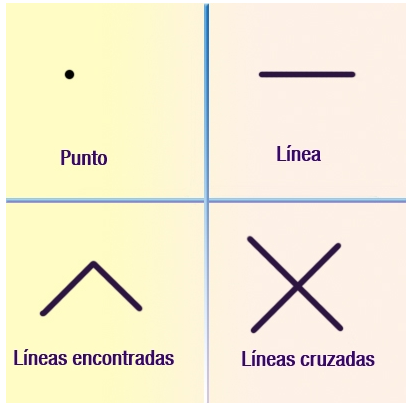
\includegraphics[scale=0.32]{el-punto.png}
    \end{figure}

    \item \textbf{Línea}: la línea no es visible por sí sola en la naturaleza. Es el resultado del movimiento de un punto que se desplaza por una superficie. La línea tiene largo pero no ancho y tiene dirección y posición. Esta limitad por dos puntos siendo esta la distancia más corta entre ambos. La línea delimita el espacio dando lugar a formas, representa el perfil o contorno de las cosas.

    \begin{figure}[H]
        \centering
        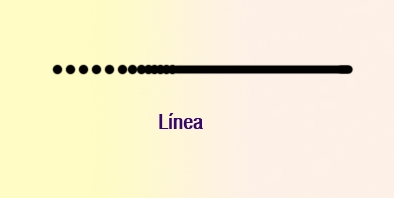
\includegraphics[scale=0.35]{la-linea.png}
    \end{figure}

    \item \textbf{Plano}: es el resultado del movimiento de una línea en dirección contraria a la suya. Un plano tiene largo y ancho pero no alto. Es la porción de superficie limitada por una línea cerrada. Define los límites extremos de un volumen.

    \begin{figure}[H]
        \centering
        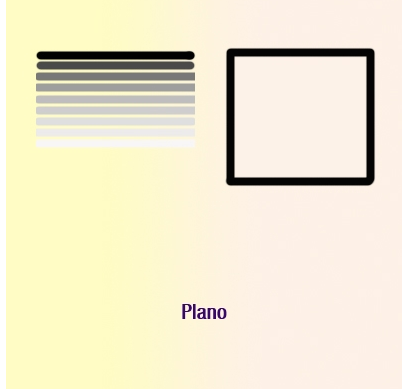
\includegraphics[scale=0.35]{el-plano.png}
    \end{figure}

    \item \textbf{Volumen}: es el resultado del movimiento de un plano que se desplaza en un dirección diferente a la suya. Tiene una posición en el espacio y esta limitado por planos. En un diseño bidimensional, el volumen es ilusorio.

    \begin{figure}[H]
        \centering
        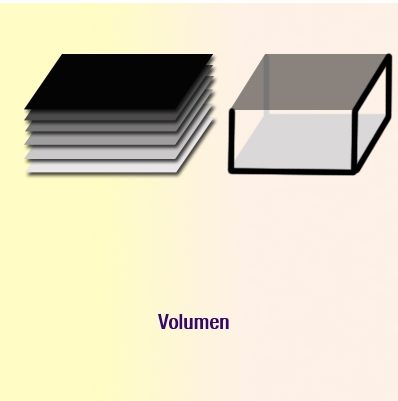
\includegraphics[scale=0.35]{el-volumen.png}
    \end{figure}
\end{itemize}

\subsection{Elementos Visuales: Forma, Medida, Color y Textura}
Los \textbf{elementos visuales} son la parte más importa de un diseño, porque son realmente lo que vemos.

Cuando dibujamos una línea en un papel empleamos una línea visible para representar la línea conceptual. Ésta tiene largo y ancho, y su color y textura vendrán determinados por el material empleado para representarla. Así, cuando lo elementos conceptuales se hacen visibles, estos tendrán color, textura, forma y medida.

\begin{itemize}
    \item \textbf{Forma}: identificamos lo que percibimos porque los que vemos posee una forma. Una forma se define como un área que se destaca del espacio que la rodea debido a un límite definido explícita o implícitamente.

    \begin{figure}[H]
        \centering
        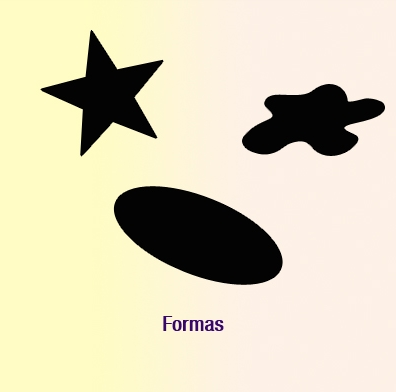
\includegraphics[scale=0.35]{la-forma.png}
    \end{figure}

    La formas pueden encontrarse entre sí de diferentes maneras:

    \begin{enumerate}[label=(\alph*)]
        \item \textbf{Distanciamiento}: ambas formas están separadas entre sí.
        \item \textbf{Toque}: si las acercamos anulamos el espacio entre ellas hasta tocarse.
        \item \textbf{Superposición}: si las acercamos aún mas, una se cruza encima de la otra.
        \item \textbf{Penetración}: igual que \textbf{(c)} pero ambas aparecen transparentes, no hay arriba y abajo y los contornos siguen siendo visibles.
        \item \textbf{Unión}: igual que \textbf{(c)} pero ambas formas quedan reunidas y se convierten en una nueva forma.
        \item \textbf{Sustracción}: cuando una forma negativa se cruza con una forma positiva.
        \item \textbf{Intersección}: igual que \textbf{(d)} pero solamente vemos la porción donde las formas se cruzan.
        \item \textbf{Coincidencia}: si acercamos las formas hasta coincidir, obtenemos una única forma.
    \end{enumerate}

    \begin{figure}[H]
        \centering
        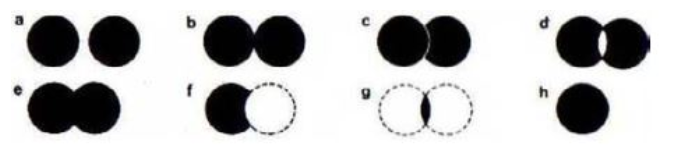
\includegraphics[scale=0.50]{la-forma-encuentro.png}
    \end{figure}

    \item \textbf{Medida}: todas las formas tienen un volumen o una dimensión. El tamaño de las formas se puede establecer de forma relativa, por comparación de unas con otras, pudiendo así decir que una forma es más grande o pequeña que otra, pero en cualquier caso, es físicamente medible.

    \begin{figure}[H]
        \centering
        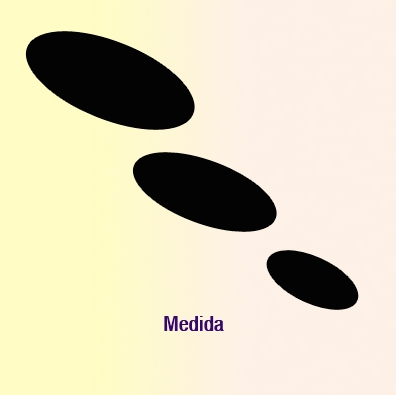
\includegraphics[scale=0.35]{la-medida.png}
    \end{figure}

    \item \textbf{Color}: todo lo que vemos en el mundo tiene color. Las cosas que vemos no solo se diferencia por su forma o tamaño, sino también por su color. El color, y el contraste de color en particular, se usa para llamar la atención sobre una parte determinada de una imagen.

    \begin{figure}[H]
        \centering
        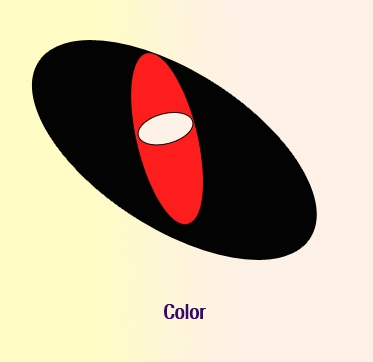
\includegraphics[scale=0.35]{el-color.png}
    \end{figure}

    \item \textbf{Textura}: es la característica visual o táctil de todas las superficies. El material con el que se hacen los objetos le aporta unas determinadas características como rugosidad, suavidad, aspereza, homogeneidad, etc...

    \begin{figure}[H]
        \centering
        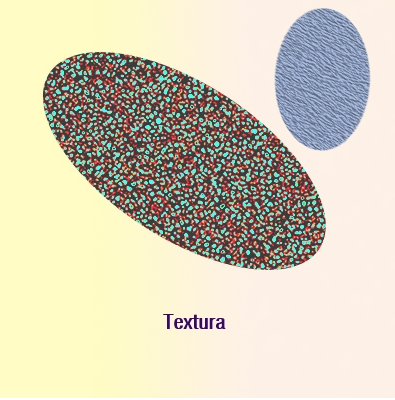
\includegraphics[scale=0.35]{la-textura.png}
    \end{figure}
\end{itemize}

\subsection{Elementos de Relación: Dirección, Posición, Espacio y Gravedad}
Este grupo de elementos gobierna la ubicación y la interrelación de las formas que componen un diseño. Algunos como la posición y la dirección pueden ser percibidos mientras que otros como el espacio o la gravedad se pueden sentir.

\begin{itemize}
    \item \textbf{Dirección}: la dirección de una forma depende de su relación con el observador, el marco que la contiene o con otras formas cercanas con cuales se compara.

    \begin{figure}[H]
        \centering
        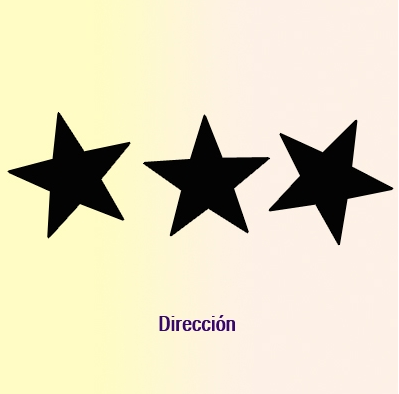
\includegraphics[scale=0.35]{la-direccion.png}
    \end{figure}

    \item \textbf{Posición}: la posición de una forma es juzgada respecto al cuadro que la contiene o la estructura global del diseño.

    \begin{figure}[H]
        \centering
        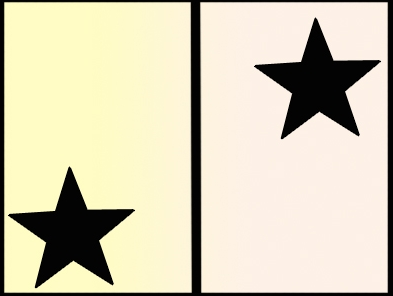
\includegraphics[scale=0.35]{la-posicion.png}
    \end{figure}

    \item \textbf{Espacio}: las formas, por muy pequeñas que sean, siempre ocupan un espacio. Así, el espacio puede estar ocupado o vacío. Se puede usar la perspectiva para simular o sugerir la ilusión de profundidad. Se pueden superponer objetos de forma que el observador perciba como más cercano el que esta delante de los demás. También podemos lograr la profundidad en el campo visual con la utilización de contraste y la variación de tamaño de las formas.

    \begin{figure}[H]
        \centering
        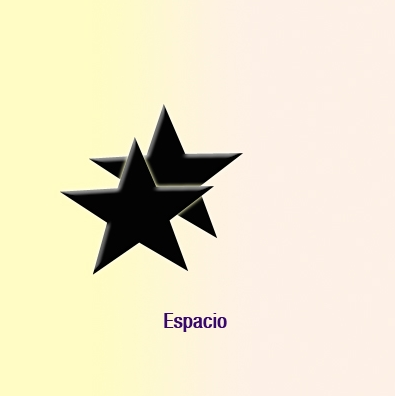
\includegraphics[scale=0.40]{el-espacio.png}
    \end{figure}

    \item \textbf{Gravedad}: la sensación de gravedad no es visual, sino psicológica. Tendemos a aplicar cualidades tales como pesadez o ligereza, estabilidad o inestabilidad, tanto a las formas individuales como a los grupos de formas.

    \begin{figure}[H]
        \centering
        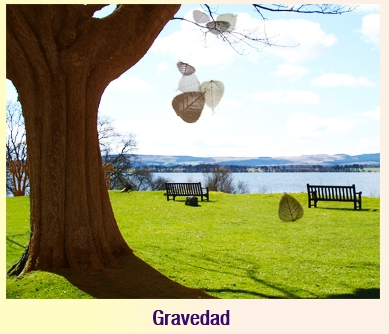
\includegraphics[scale=0.35]{la-gravedad.png}
    \end{figure}
\end{itemize}

\subsection{Elementos Prácticos: Representación, Significado y Función}
Los elementos prácticos del diseño permanecen ocultos en el contenido y la trascendencia del diseño. Estos elementos son:

\begin{itemize}
    \item \textbf{Representación}: una forma es representativa cuando se deriva del mundo natural o del mundo hecho por el ser humano. la representación puede ser \textbf{realista}, \textbf{estilizada} o \textbf{medio abstracta}. Una fotografía de un documento es una representación realista del mismo. Un dibujo de los perfiles de dicho documento es una representación estilizada. Un dibujo naif de dicho documento es una representación medio abstracta.

    \begin{figure}[H]
        \centering
        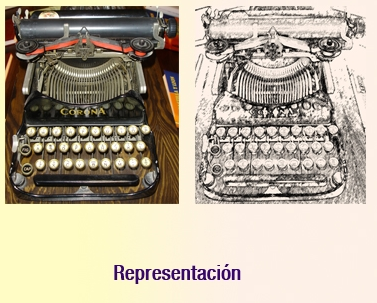
\includegraphics[scale=0.45]{la-representacion.png}
    \end{figure}

    \item \textbf{Significado}: es la imagen conceptual que se representa en nuestra mente cuando el diseño transporta un mensaje visual. Cada receptor del mensaje dará una interpretación y un significado distinto, según sean sus conocimientos y experiencias.

    \begin{figure}[H]
        \centering
        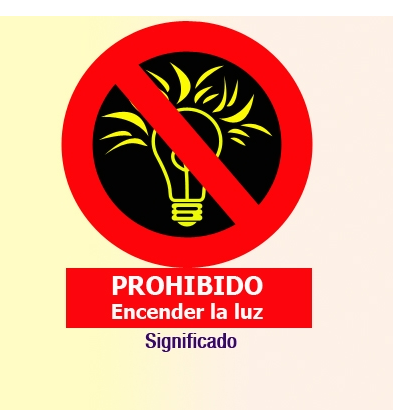
\includegraphics[scale=0.40]{el-significado.png}
    \end{figure}

    \item \textbf{Función}: la función se hace presente cuando un diseño debe servir a un determinado propósito. La imagen anterior, por ejemplo, cumple una función muy importante. Colocada en el lugar adecuado, como una sala de revelado, cumple la función de mantener el ambiente oscuro para poder trabajar.
\end{itemize}

\section{Interfaces Web}
El número de usuario de internet aumenta día a día, y el número de páginas Web también. Internet a cambiado, no solo la forma de trabajar sino también la forma en la que nos relacionamos.

Creamos páginas web para poder comunicar cosas a través de internet. Creamos páginas de tipo personal donde publicamos nuestras opiniones, nuestras fotos, nuestros viajes, etc. También creamos páginas con las que pretendemos obtener algún beneficio económico.

Todas y cada una de estas páginas son creadas con alguna finalidad. Lograr nuestro objetivo dependerá en gran medida de la eficacia del diseño que realicemos.

En \href{https://es.wikipedia.org/wiki/World_Wide_Web}{esta entrada de Wikipedia} tiene información importante que debes conocer sobre la \textbf{World Wide Web}, como su historia, estándares y tecnologías. Debes consultar también los enlaces de cada uno de los estándares.

\subsection{Interacción Persona-Ordenador}

La \textbf{IPO} (Interacción Persona-Ordenador) es la disciplina que estudia el intercambio de información entre personas y ordenadores. Cuando hay una buena interacción entre el usuario y ordenador el intercambio de información es más eficiente, hay menos errores y la satisfacción de la persona es mayor.

Hoy en día la mayor parte de los sistemas informáticos son interactivos y su éxito radica en gran medida en la eficacia del diseño de la interfaz persona-ordenador. Por ello, la interfaz debe estar diseñada pensando en las necesidades del usuario.

Debemos tener en cuenta que cada día es mayor el número de personas que utiliza el ordenador, y que estas personas se enfrentan a este tipo de interacción con diferentes niveles de formación y perspectiva.

\subsection{Diseño de una Interfaz Web: Objetivos}
Una \textbf{interfaz Web} es un \textbf{sistema gráfico} que permite a los usuarios acceder a los contenidos de la Web mediante diferentes elementos gráficos, los cuales son conocidos por la gran mayoría de usuarios que accederán a nuestra web.

El \textbf{objetivo principal} en el diseño de una interfaz Web es que sus usuarios puedan acceder a todos los contenidos de la forma más rápida y simple posible.

Para que el \textbf{diseño web} sea \textbf{efectivo}, debemos diseñar una interfaz que cobra todos nuestros objetivos. Este diseño debe facilitar que nuestros usuario puedan acceder con facilidad a todo el contenido, puedan interactuar con eficacia con todos sus componente y de forma satisfactoria.

Para conseguir dicho objetivo debemos tener en cuenta las siguiente pautas:

\begin{itemize}
    \item La paciencia de las personas no es ilimitada. Si una persona entra en una web y no encuentra rápidamente la información que esta buscando no permanecerá mucho tiempo.
    \item El gusto, considerado como una cuestión de preferencias estéticas, varia mucho de una persona a otra, pero no debemos olvidar que un diseño cuidadoso, una interfaz agradable y un uso coherente de los elementos gráficos nunca nos hará perder usuarios.
    \item Los enlaces que no funcionan o que no redirigen a la información que prometían generan en el visitante una sensación de rechazo, con la consiguiente perdida de confianza en nuestra página, llegando incluso a la determinación de no volver a visitarla de nuevo.
\end{itemize}

A la hora de \textbf{realizar el diseño} de una página web existen \textbf{diferentes filosofías} o \textbf{estrategias}. Nosotros vamos a comentar las dos más empleadas actualmente:

\begin{itemize}
    \item \textbf{Diseño Responsivo o Adaptativo}: hoy en día cuando diseñamos una aplicación debemos pensar que ésta no se va solo a visualizar en un mismo tipo de dispositivo, así que cuando la estamos diseñando tenemos que tener en cuenta los diferentes tipos de dispositivos en los que se va a visualizar. Habitualmente se desarrolla la página web primero para un ordenador y posteriormente tenemos que indicar como se va a visualizar esta en otros dispositivos como tablets, móviles, etc. Dichos cambios pueden consistir en modificar o cambiar el aspecto, o incluso en eliminar algunos elementos del diseño.

    \item \textbf{Diseño Mobile First}: actualmente esta cambiando la tendencia sobre visualización de contenido web, y mientras durante mucho tiempo las webs se han visualizado el ordenador como dispositivo principal, actualmente son los dispositivos móviles donde más páginas web se ven. Teniendo en cuenta esto, lo que persigue esta filosofía es realizar el diseño primero para un dispositivo móvil y posteriormente realizar las modificaciones oportunas para que se adapte a otro tipo de dispositivos como ordenadores.
\end{itemize}

\subsection{Características: Usable, Visual, Educativa y Actualizada}
Cuando diseñamos una web, debemos tener en cuenta como siente o como perciben los seres humanos. Si, por ejemplo, nuestra web ofrece cursillos a las personas de la tercera edad, debemos tener en cuenta las limitaciones que pueden tener este grupo de personas, como problemas de visión y audición. Mientras que si nuestro sitio web va enfocado al público infantil deberemos cuidar más la decoración e incluso abusar de colores llamativos.

Hay características que son deseables en un sitio web y características que son imprescindibles. Determinar cuales son deseable y cuales imprescindibles dependerá en gran medida del público al que vaya dirigido nuestro sitio web, aunque unas de las características que deberíamos considerar siempre imprescindibles es \textbf{la usabilidad}.

\textbf{Usable} es un termino ampliamente utilizado en el mundo informático. Es una traducción del termino inglés ``Useable'' y por analogía con el termino español ``utilizable'' podemos definirlo como ``\textbf{que se puede usar}''. Podríamos pensar que un sitio web es usable simplemente por poder acceder a él y haber visitado alguno de sus enlaces. Pero nada más lejos de la realizar, un \textbf{sitio we es usable} si al usuario le resulta \textbf{fácil} el \textbf{uso de su interfaz}.

La popularidad de un sitio web depende en gran parte de su aspecto visual. Podemos decir que un sitio web es visual cuando las percepciones del usuario, sus opiniones acerca del sitio, y sus sentimientos y actitudes generados mientras lo usa, son positivos. Un \textbf{sitio web debe ser atractivo} para mantener la atención del usuario, pero también debe ser coherente en el uso de los elementos gráficos.

Un sitio web \textbf{es visual} cuando los elementos gráficos empleados están orientados a conseguir los objetivos del sitio y no se han empleado como elementos decorativos.

Tenemos además que tener en cuenta que las personas desarrollan modelos como resultado de sus experiencias y emplean estos modelos para almacenar información y conocimiento. Una interfaz \textbf{es educativa} cuando es fácil de aprender por el usuario. La \textbf{facilidad de aprendizaje} es una medida de la \textbf{cantidad de tiempo} necesaria para \textbf{conocer la interfaz} a través de su uso y, también es una medida de la cantidad de tiempo que el usuario \textbf{retiene ese conocimiento} sin necesidad de usar la interfaz.

Si no queremos perder popularidad entre nuestro visitantes habituales, es conveniente ofrecer periódicamente nuevos contenidos que le puedan interesar. Es importante \textbf{actualizar periódicamente} nuestro sitio Web. Podemos actualizarlo diariamente, semanalmente, mensualmente, etc. Dependerá del sitio web y los servicios que ofrezcan. Pero también es importante \textbf{actualizar la interfaz} modificando aquellos elementos que puedan lograr que sea aún más usable, visual y educativa.

\subsection{Componentes de Una Interfaz Web}
Dado que la interfaz Web es el medio de comunicación entre los usuarios y el sitio web que visitan, debemos tener claros cuales son los elementos que compondrán nuestra interfaz. Todos elementos deberán permitir al usuario identificar la función que desempeñan de forma que pueda acceder a todos los contenidos sin tener que realizar extraños razonamientos.

Son muchos los elementos de los que pueda estar compuesta nuestra interfaz Web. El número de elementos utilizados dependerá de la finalidad del sitio. Así, un portal de noticias o de un organismo oficial usarán más elementos que el sitio de un restaurante o una página web personal. Los \textbf{elementos} más destacados que podemos encontrar en cualquier de ellos son:

\begin{itemize}
    \item Elementos de \textbf{Identificación}: son aquellos elementos que identifican plenamente el sitio Web. El usuario, a la vista de estos elementos, debe saber a quién pertenece la web. Por ejemplo, el logo de la página, el título de ésta, etc...
    \item Elementos de \textbf{Navegación}: son aquellos que están presentes en cada una de las pantallas de un sitio web y permiten al usuario moverse por las diferentes secciones del sitio y retomar de nuevo la portada. Estos elementos deben ser lo suficientemente intuitivos para que el usuario sepa que hay que hacer para acceder al contenido. Un ejemplo son los diferentes enlaces del sitio, barras de navegación, etc...
    \item Elementos de \textbf{Contenidos}: son las zonas en las que se muestra la información relevante de cada una de las páginas que componen el sitio. Dentro de una zona de contenido se debe distinguir la zona del Título del Contenido y el Contenido propiamente dicho. Por ejemplo, una noticia, una entrada de un blog, etc...
    \item Elementos de \textbf{Interacción}: son las zonas del sitio Web donde se ofrece la realización de acciones a los usuarios. Ejemplos son las barras de búsqueda, los formularios, etc...
\end{itemize}

\subsubsection{Zona de Navegación}
Como hemos dicho, los elementos de navegación son los que nos permiten acceder a todos los contenidos que se encuentran en las diferentes páginas que componen el sitio Web. Pero lo que no hemos dicho, es que si queremos que nuestra Web sea usable, el usuario debe conseguir poder navegar por la página sin perderse. Para conseguirlo, el sistema de navegación debería tener los siguiente elementos:

\begin{itemize}
    \item Elementos de \textbf{regreso a la portada}.
    \item \textbf{Menú de secciones} o de áreas de interés.
    \item \textbf{Información} sobre la \textbf{ubicación del usuario} dentro de sitio.
\end{itemize}

Es importante para el usuario tener algún \textbf{elemento} que le permita \textbf{volver al principio} sin necesidad de usar la herramienta ``ir hacia atrás'' del navegador. Es problema suele resolverse \textbf{empleando un enlace} en el \textbf{logotipo} de la empresa que se sitúa normalmente en la parte superior izquierda de cada una de las páginas que componen el sitio.

El \textbf{menú de secciones} es una zona de la interfaz donde se detallan las secciones y/o áreas en las que está dividida la información contenida en el sitio Web. Debe ser fácilmente localizable y se suele ubicar en la parte superior de cada página, debajo del logotipo. Es importante que estas secciones estén bien identificadas mediante un texto o imagen descriptiva. También es importante que mantenga la posición en todas las páginas que componen el sitio.

No debemos olvidar que cuando el sitio Web es suficientemente grande, con muchas secciones y subsecciones, es de gran importante que el \textbf{usuario sepa} en todo momento el lugar en el que se encuentra dentro del sitio. Por ello debemos informar, en cada una de las páginas de contenido, el camino recorrido desde la página principal hasta la página actual, y lo haremos mediante una línea de texto por encima del menú de secciones o de la zona de contenidos. Podemos aprovechar esta línea para permitir, mediante el uso de enlaces, vueltas hacia atrás en el camino de navegación. Esto es lo que se denomina como técnica de navegación de \textbf{migas de pan} o \textbf{breadcrumb}.

En la siguiente imagen, podemos ver los diferentes elementos que acabamos de mencionar en la Web del Ministerio de Educación y Ciencia.

\begin{figure}[H]
    \centering
    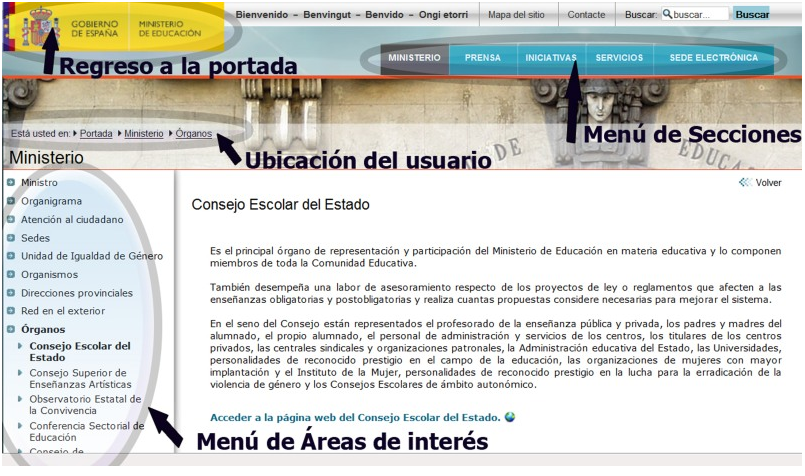
\includegraphics[scale=0.45]{elementos-navegacion.png}
    \caption{Elementos de navegación}
\end{figure}

\subsubsection{Zona de Contenido e Interacción}
El \textbf{contenido} es la \textbf{parte esencial} de una página Web. Es importante que los contenidos estén escritos en un lenguaje claro y conciso, y presentados en un formato agradable y de fácil lectura. Además, si el sitio Web esta formado por diferentes páginas, el contenido debe situarse siempre en la misma posición. También es importante evitar que el usuario tenga que realizar grandes desplazamientos durante la lectura o visualización del contenido. Siempre es mejor dividir el contenido en varias páginas y enlazar una con otra.

Cuando el usuario está navegando por un sitio Web y eligiendo los enlaces que quiere visitar de la página web está interactuando con ésta, pero no es a este tipo de interacción al que nos referimos, sino que nos referimos a otras \textbf{zonas de interacción} donde el usuario \textbf{participa} de alguna manera. Cuando el usuario selecciona el idioma en el que quiere ver la página, realiza una búsqueda usando un formulario, cuando envía una opinión o cuando firma un libro de visitas. Todos los elementos del sitio necesarios para la realización de este tipo de acciones forman parte de la \textbf{zona de interacción}.

En la siguiente imagen imagen podemos ver la misma Web de la figura anterior con las zonas de contenido e interacciones señaladas.

\begin{figure}[H]
    \centering
    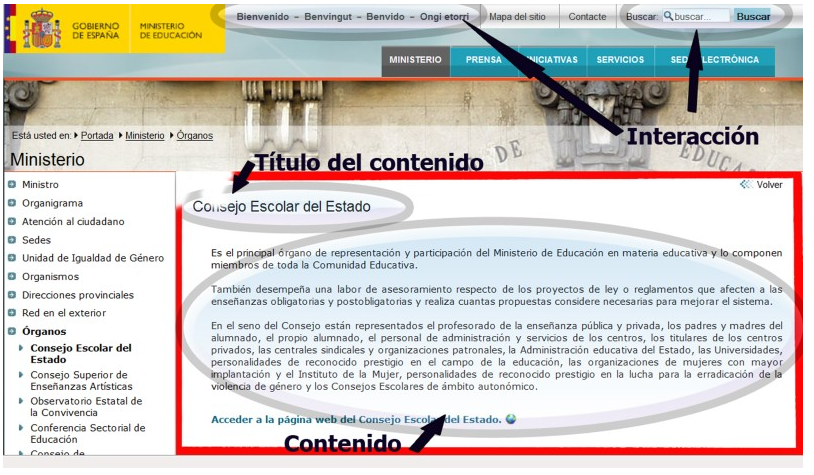
\includegraphics[scale=0.45]{elementos-contenido.png}
    \caption{Elementos de contenido e interacción}
\end{figure}

Hay muchos \textbf{elementos que permiten la interacción} y cada uno de ellos cumple una función muy concreta. Algunos de ellos son los siguientes:

\begin{itemize}
    \item \textbf{Botón}: elemento que permite al usuario realizar una acción. Se puede usar para su representación un rectángulo con efecto de relieve y con un texto que sirve para orientar al usuario sobre la función de dicho botón. Su diseño debe mantenerse en todo el sitio web.

    \item \textbf{Áreas de Texto}: son rectángulos en los que el usuario puede escribir. Deben ir acompañados de una etiqueta que indique el contenido que se le pide al usuario.

    \item \textbf{Botones de Opción}: son elementos excluyentes entre sí que están agrupados bajo una misma descripción. Constan de unas circunferencias acompañadas de un texto descriptivo. Se identifica el que esta seleccionado porque tiene un círculo negro.

    \item \textbf{Casillas de Verificación}: al contrario que los botones de opción, estás no son excluyentes entre sí. El usuario puede no seleccionar ninguna o seleccionar una, alguna o todas las casillas. Suelen ir también agrupadas bajo una misma descripción y acompañadas de un texto descriptivo. Tienen forma de cuadrado y cuando se seleccionan se marcan con una ``X'' o una ``V''.
\end{itemize}

\subsection{Maquetación Web}
Según la RAE, una \textbf{maqueta} es un boceto previo a la composición de un texto que se va a publicar, usado para determinar sus características definitivas. También define un \textbf{boceto} como esquema o proyecto en el que se bosqueja cualquier obra.

A la hora de realizar la maquetación web debemos tener en cuenta:

\begin{itemize}
    \item Cuáles son \textbf{los elementos} que van a contener cada página de nuestro sitio Web.
    \item Como irán \textbf{colocados} cada uno de esos elementos dentro de de las páginas teniendo en cuenta siempre el espacio disponible, es decir, la ventana del navegador.
\end{itemize}

Si hemos hablado con el cliente tendremos los datos necesarios para la realizar una serie de bocetos preliminares de lo que será nuestro sitio web. Además, hay que tener en cuenta, que un boceto también refleja la \textbf{interactividad} y \textbf{funcionalidad} del sitio Web.

Para \textbf{diseñar un sitio Web} debemos comentar realizan una distribución de los grandes bloques de elementos de información. Se debe tener en cuenta en el diseño a todas las páginas web que componen el sitio. Todas deben manejar la misma estructura. Este tema los volveremos a ver al final de esta unidad cuando hablemos de las plantillas de diseño.

\subsubsection{Elementos de Ordenación}
Cuando diseñamos una web debemos de ser consistentes en las distribución de los grandes bloques de información en todas las páginas que componen el sitio Web, teniendo además en cuenta el espacio disponible en la ventana del navegador.

Además de los bloques que hemos visto ya, como las zonas de navegación, contenido e interacción, podemos encontrar otros bloques, los cuales podemos ver en la siguiente figura.

En ella podemos ver un boceto de la colocación de los diferentes bloques de información. A continuación, explicaremos un poco sobre cada uno de ellos haciendo especial hincapié en los que aun no hemos comentado en puntos anteriores.

\begin{figure}[H]
    \centering
    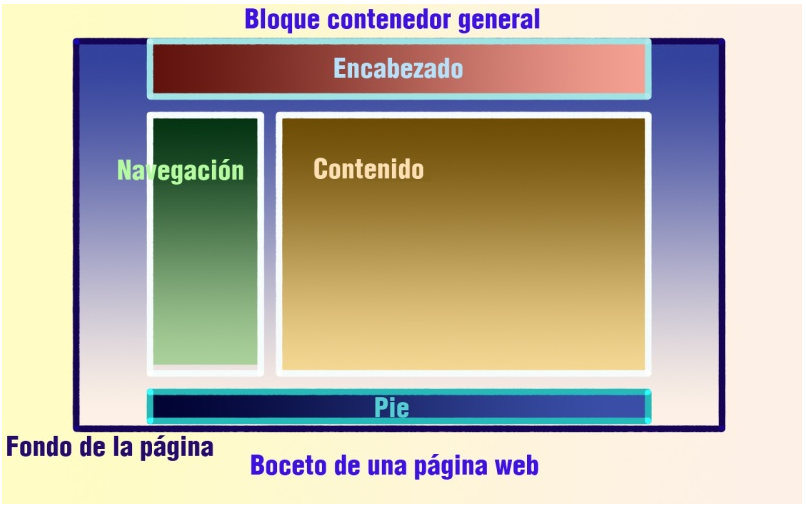
\includegraphics[scale=0.45]{boceto-bloques.png}
    \caption{Elementos de Ordenación}
\end{figure}

El \textbf{Bloque de Encabezado} esta siempre situado en la parte superior de cualquier página. Suele contener además de los elementos identificativos de la página web: el logotipo, nombre de la empresa, elementos de acción que permiten cambiar el idioma de lectura, realización de búsquedas, e incluso si el sitio es grande, elementos de navegación que permanecen a la vista en todas las páginas. Éste se \textbf{repite en todas las páginas} del sitio Web y debe ser visible en todas ellas siempre que sea posible y la complejidad del sitio nos lo permita.

El \textbf{Bloque de Navegación} es donde se coloca el sistema de navegación del que ya hemos hablado en el apartado  de Zonas de Navegación e Interacción.

El \textbf{Bloque de Contenido} es aquel en el que se muestran los contenidos. Los contenido representan la meta del usuario y la razón por la que visita nuestro sitio Web, por lo que debemos prestar mucha atención al diseño de este bloque. Debemos reservar una zona lo suficientemente grande como para que el usuario pueda leer el contenido cómodamente, sin necesidad de realizar grandes desplazamientos. Es \textbf{importantísimo} que el usuario \textbf{no tenga} que realizar \textbf{desplazamientos horizontales} para leer el final de cada línea.

El \textbf{Bloque de Pie de Página} esta situado al final de la página y al igual que en encabezado se suele repetir en todas las páginas del sitio Web. Normalmente se emplea como zona de \textbf{navegación complementaria} a la zona superior situada en el encabezado. En ellas se suelen repetir algunos enlaces que se colocan en el encabeza como Mapa del sitio del web. o el enlace de información de contacto, y además, se colocan algunos enlaces nuevos como las información relativa a los derechos de autor, privacidad, información lega, etc...

El diseño del pie no suele ser tan elaborado como el encabezado, ya que si importancia es menor. El usuario debe ser consciente que lo que está viendo es el pie. Esto es de especial importancia en aquellos casos en los que por ser el tamaño vertical de la página mayor que la ventana del navegador, el usuario se ve obligado a desplazarse verticalmente, pudiendo perder de vista el encabezado. Con un diseño más sencillo del pie respecto del resto de bloques conseguimos esa percepción por parte del usuario.

\subsection{Mapa de Navegación}
Cuando un sitio es muy grande y complejo, conviene tener un mapa del sitio que ayude a los usuarios a encontrar lo que buscan. En nuestro ejemplo, la página de portada permite consultar el mapa del sitio tanto en el encabezado como en el píe de página. Una vez pulsado en el enlace del mapa, verás la imagen que se muestra a continuación.

\begin{figure}[H]
    \centering
    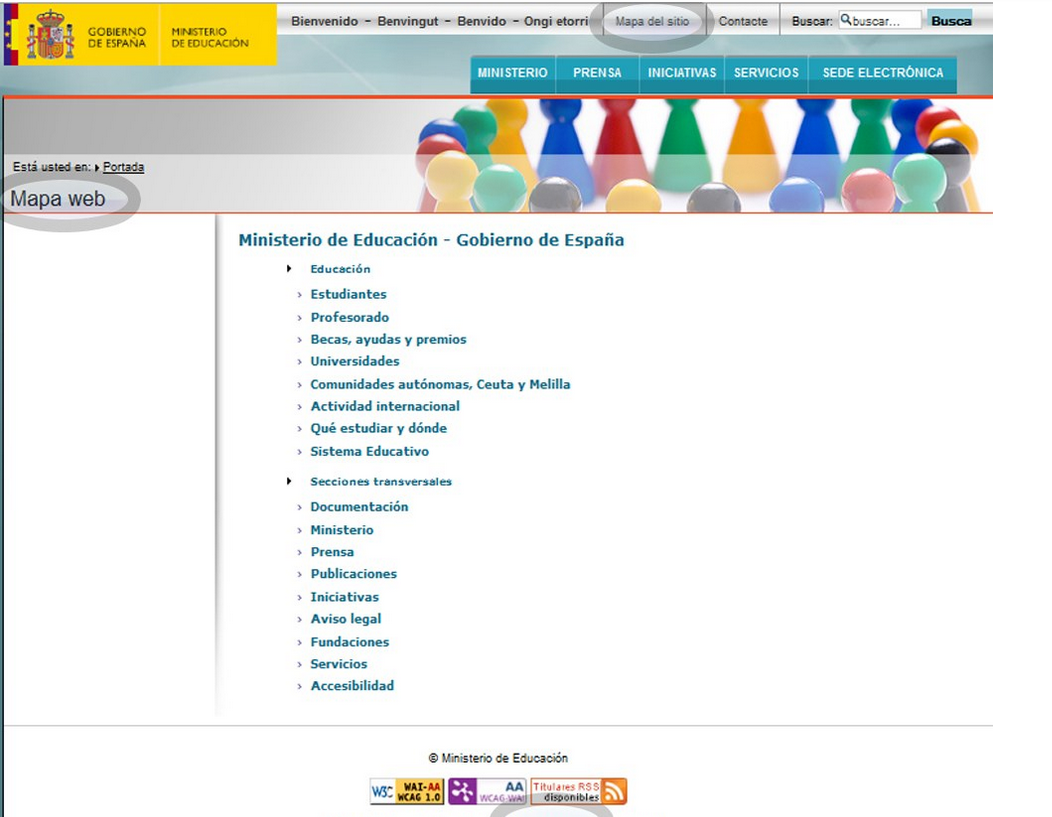
\includegraphics[scale=0.35]{mapa-sitio.png}
    \caption{Mapa del sitio de la web del Ministerio de Educación}
\end{figure}

El \textbf{Mapa del Sitio} proporciona a los visitantes un lugar donde buscar de forma sencilla los contenidos que le interesan si es que no los ha encontrado en la página principal.

La \textbf{obligación de crear un mapa} es directamente proporcional al \textbf{tamaño y la complejidad} del sitio Web. Así, si nuestro sitio consta de una sola página donde hay enlaces a páginas ajenas, no será necesario poner un enlace al Mapa del Sitio. Si por el contrario nuestro sitio consta de una página principal con enlaces a secciones que a su vez están divididas en subsecciones, se sería conveniente crear una Mapa del Sitio y poner un enlace a él en la portada.

En los siguientes enlaces puedes ver diferentes mapas del sitio de páginas web de algunas comunidades autónomas así como del Ministerio de Educación, que ya hemos visto antes:

\begin{itemize}
    \item \href{https://sede.comunidad.madrid/buscador?t=&tipo=All&consejeria=All&estado_pendiente%5B1%5D=1&estado_plazo%5B1%5D=1&estado_tramitacion%5B1%5D=1}{Mapa de la web de la Comunidad Autónoma de Madrid}
    \item \href{https://www.xunta.gal/mapa-do-portal}{Mapa del sitio de la Xunta de Galicia}
    \item \href{https://web.gencat.cat/es/ajuda/mapaweb/}{Mapa del sitio de la web de la Generalitat de Catalunya}
\end{itemize}

Seria interesante que ademas de estos mapas consultes por tu cuenta los de otras webs para ver los diferentes diseños que te puedes encontrar referentes al mapa del sitio web.

\subsubsection{Prototipos de Mapas de Navegación}
Ahora que ya sabes que es un mapa de navegación vamos a ver los tipos de mapas más comunes que nos podemos encontrar.

El Mapa de un sitio Web va a tener una estructura que dependerá de la relación que tengan las páginas del sitio entre ellas. Esta relación puede ser:

\begin{itemize}
    \item \textbf{Lineal}
    \item \textbf{Reticular}
    \item \textbf{Jerárquica}
    \item \textbf{Lineal Jerárquica}
\end{itemize}


\begin{figure}[H]
    \centering
    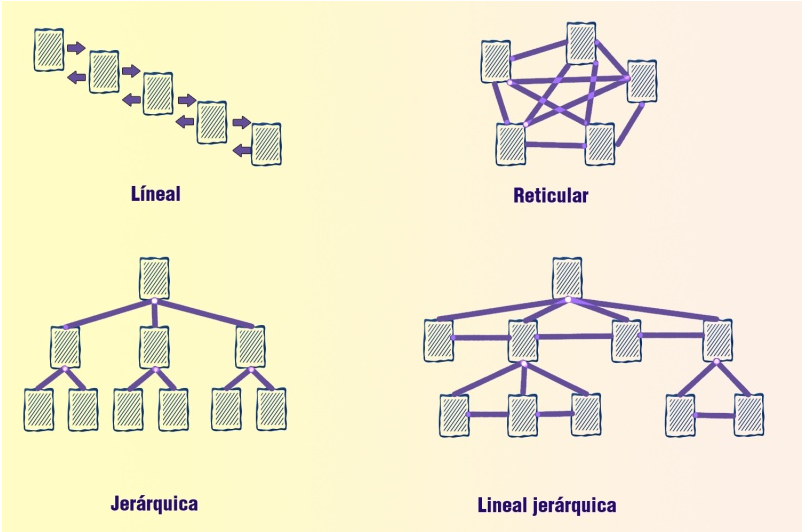
\includegraphics[scale=0.45]{mapa-sitio-estructura.png}
    \caption{Estructuras de Mapas del Sitio}
\end{figure}

En la anterior imagen podemos ver de una forma más gráfica los diferentes tipos de estructura que nos podemos encontrar, pero para que quede claro, vamos a explicar un poco cada unos de ellos:

\begin{itemize}
    \item \textbf{Estructura Lineal}: es adecuada en aquellos sitios donde la lectura de las páginas se hace de manera secuencia. Su estructura es similar a la de un libro donde avanzar de página en página, pero puedes volver a la página anterior, y desde esta a la anterior, para releer algún párrafo.

    \item \textbf{Estructura Reticular}: se emplea en aquellos sitios en los que todas sus páginas están relacionadas entre sí. No resulta adecuado cuando el sitio es compuesto por muchas páginas ya que el usuario puede llegar a perderse.

    \item \textbf{Estructura Jerárquica}: es la más común. Se emplea en aquellos sitios donde existen varias secciones bien diferenciadas pero de poca complejidad, de modo que el usuario no tiene porque navegar de una sección a otra.

    \item \textbf{Estructura Lineal Jerárquica}: es una de las más empleadas cuando cada sección tiene un volumen de información más elevado y la lectura se realiza de forma secuencial en cada sección. También se emplea este mapa en sitios en los que sus secciones representan un grado de complejidad de la información presentada y se permite la navegación entre secciones.
\end{itemize}

\subsection{Detección de Patrones}
Un \textbf{Patrón de Diseño} es una solución a un problema concreto que se puede emplear en repetidas ocasiones en problemas similares haciendo pequeñas variaciones. Podemos distinguir dos tipos de patrones:

\begin{itemize}
    \item \textbf{Patrones de Diseño de Software}, orientados a la funcionalidad.
    \item \textbf{Patrones de Diseño de Interacción}, orientados a la usabilidad.
\end{itemize}

La finalidad de la personas que diseñan una interfaz web debe ser la de desarrollar diseños centrados en la usabilidad, la eficiencia, la eficacia y la satisfacción del usuario. Para lograrlo, se puede apoyar en los \textbf{Principio de Gestalt} como principios de organización de elementos dentro de la interfaz y aplicarlos a la creación de los patrones de diseño.

En los siguiente subapartados vamos a ver los principios de Gestalt más importantes y como se aplican estos a lo patrones de diseño web.

\subsubsection{Principios de Proximidad y Semejanza}
Los principio de proximidad y semejanza tiene que ver con como agrupa nuestra mente los elementos que están cerca o que son similares. Vamos a explicar más detalladamente cada uno de estos principios.

\begin{itemize}
    \item \textbf{Principio de Proximidad}

    Nuestra mente suelen agrupar los elementos en función de la distancia que hay entre ellos. En la siguiente figura, podemos ver un ejemplo gráfico de este principio.

    \begin{figure}[H]
        \centering
        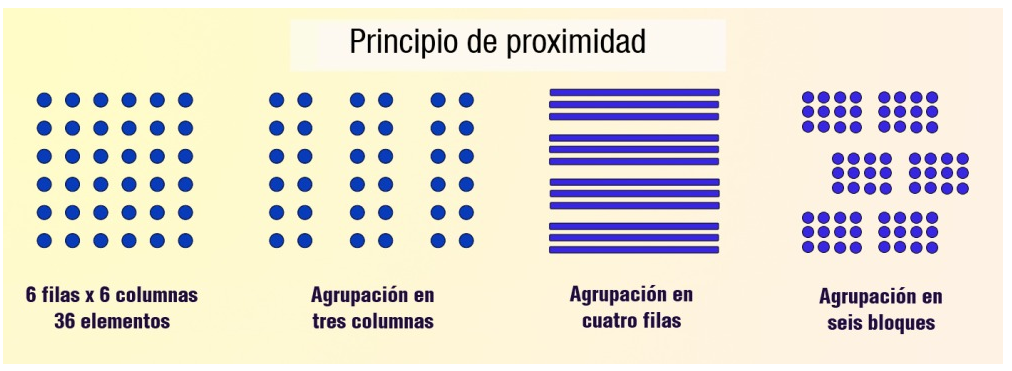
\includegraphics[scale=0.40]{principio-prox-1.png}
        \caption{Principio de Proximidad de Gestalt}
    \end{figure}

    Un ejemplo de la aplicación de este principio lo puedes ver en una de las páginas web que componen el sitio de la Comunidad de Madrid.

    \begin{figure}[H]
        \centering
        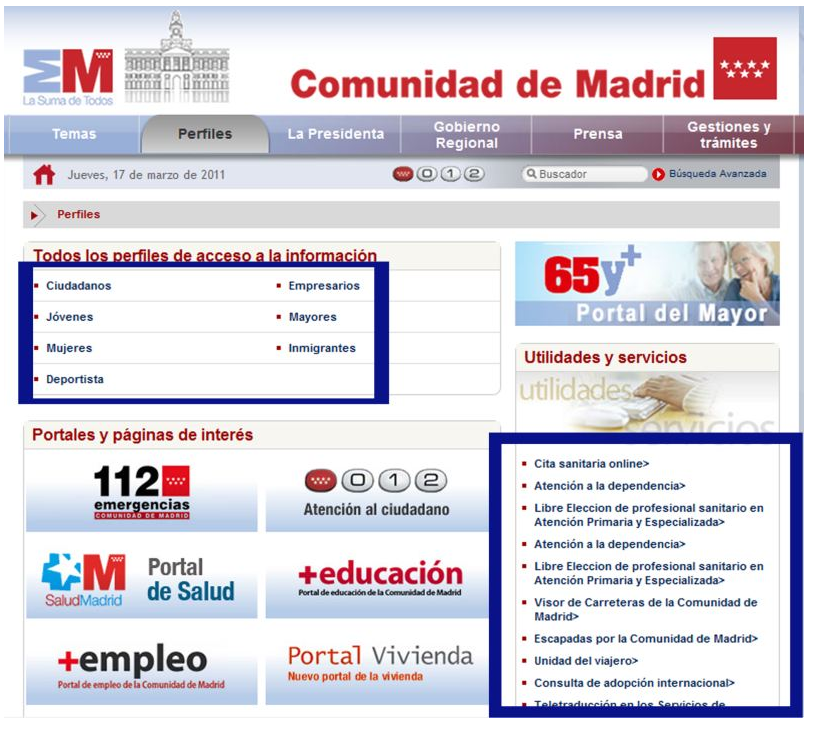
\includegraphics[scale=0.40]{principio-prox-2.png}
        \caption{Principio de proximidad en la web de la CAM}
    \end{figure}

     En esta imagen, se han agrupado dentro de dos rectángulos azules, aquellos elementos que, siendo todos enlaces a otras páginas del sitio y presentando el mismo formato, se perciben como bloques distintos por estar todos sus elementos más próximos entre sí.

     La cercanía de los elementos del mismo tipo es percibida por el usuario como una misma unidad. Y la distancia que hay entre los dos bloques, es suficiente para que el usuario los perciba como elementos que pertenecen a diferentes categorías.

     \item \textbf{Principio de Semejanza}

     Nuestra mente suele agrupar los elementos que son similares en su aspecto visual, es decir, que tiene una forma, color, tamaño, etc.., similar. En la siguiente imagen lo vemos de forma más gráfica.

     \begin{figure}[H]
         \centering
         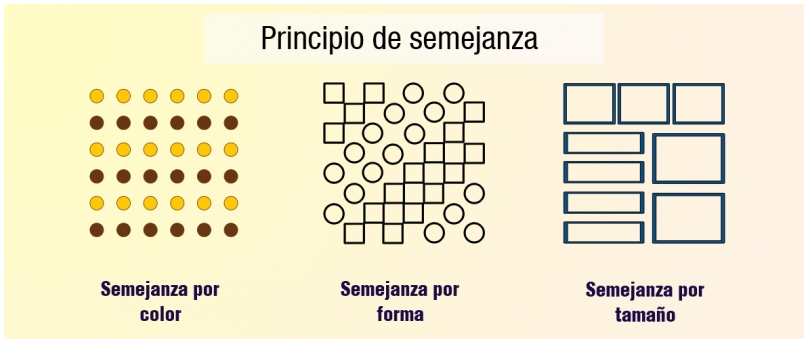
\includegraphics[scale=0.40]{principio-semej-1.png}
         \caption{Principio de semejanza de Gestalt}
     \end{figure}

    Nuestra mente no percibe 36 elementos en la parte izquierda de la imagen, sino que percibe 3 filas de elementos amarillos y 3 filas de elementos negros. En la parte central de la imagen vemos los elementos con forma similar formar la diagonal principal. En la imagen de la derecha distinguimos 3 bloques de rectángulo, el bloque superior horizontal y dos bloques verticales paralelos.

    \begin{figure}[H]
        \centering
        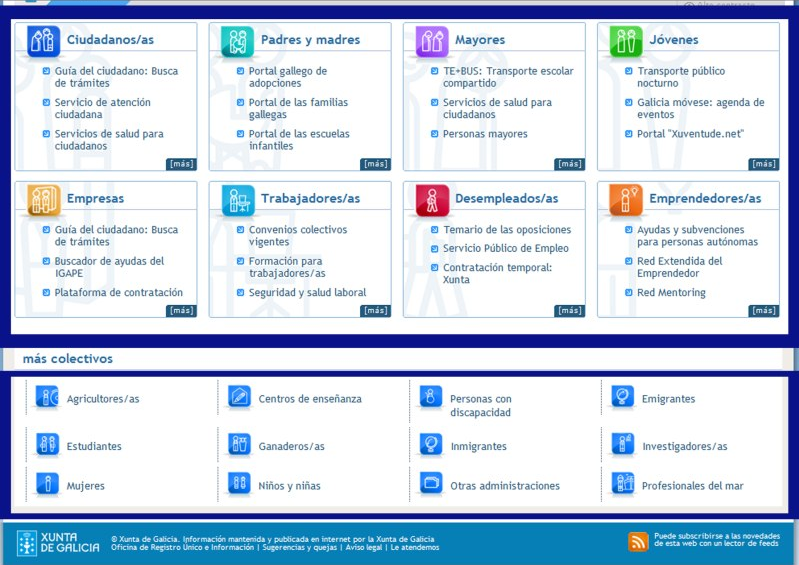
\includegraphics[scale=0.40]{principio-semej-2.png}
        \caption{Principio de semejanza en la web de la Xunta de Galicia}
    \end{figure}

    En esta imagen podemos ver un ejemplo de aplicación de este principio. Se han agrupado, dentro de rectángulos azules, los elementos que se perciben como un bloque, aunque son enlaces a diferentes páginas del sitio, son similares entre sí tanto en forma como en tamaño.
\end{itemize}

\subsubsection{Principios de Simetría y Continuidad}
Ahora vamos a ver los principios de simetría y continuidad, y como nuestra mente percibe como un todo elementos que son simétricos o que sugieren continuidad a pesar de estar ésta interrumpida.

\begin{itemize}
    \item \textbf{Principio de Simetría}

    Nuestra mente tiene a percibir como un único elemento aquellos elementos que tiene una disposición simétrica, como podemos de forma más clara en la siguiente imagen.

    \begin{figure}[H]
        \centering
        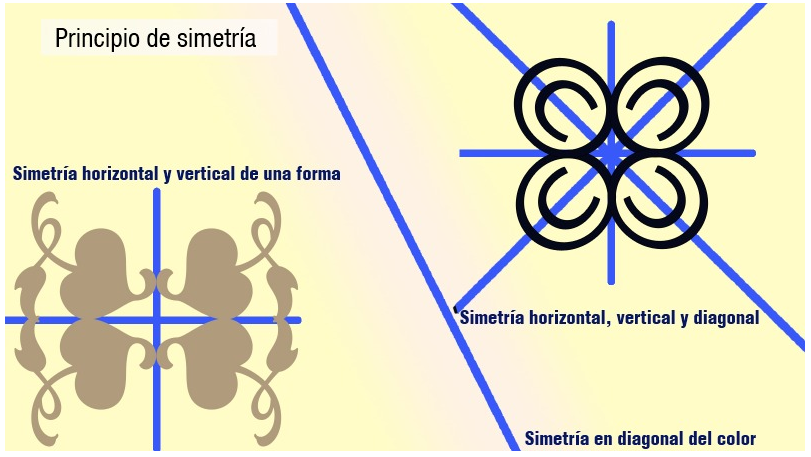
\includegraphics[scale=0.35]{principio-sim-1.png}
        \caption{Principio de simetría de Gestalt}
    \end{figure}

    En este dibujo, por ejemplo, no vemos el símbolo de copyright que está colocado cuatro veces, pero girado de forma que la C interior apunte al centro, sino que vemos una flor con cuatro pétalos.

    Un ejemplo de la aplicación de este principio lo puedes ver en la imagen la tienda online Bornay Desserts, que vemos a continuación.

    \begin{figure}[H]
        \centering
        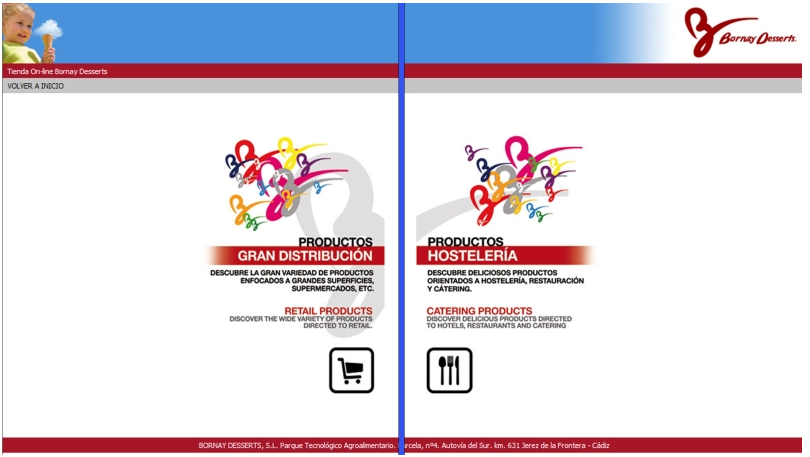
\includegraphics[scale=0.35]{principio-sim-2.png}
        \caption{Principio de simetría en la página de Bornay Desserts}
    \end{figure}

    En esta imagen se han separado, mediante una línea vertical azul, las dos zonas simétricas. En la izquierda el texto está alineado a su derecha mientras que en la izquierda éste está alineado a su izquierda. Desde lejos, parece un único elemento centrado en la imagen.

    \item \textbf{Principio de Continuidad}

    Nuestra mente tiende a percibir los elementos continuos aunque estén interrumpidos, como podemos ver en la siguiente imagen.

    \begin{figure}[H]
        \centering
        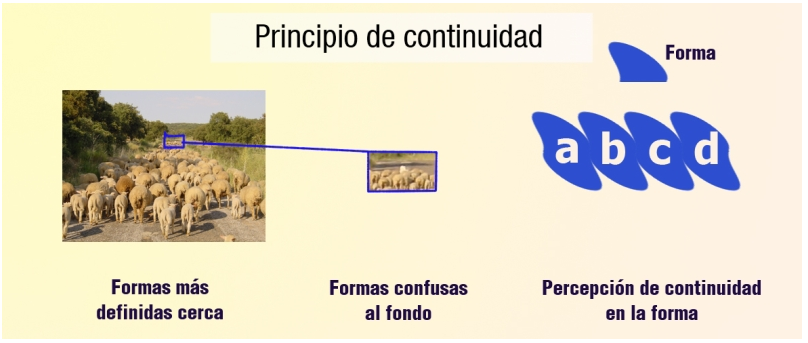
\includegraphics[scale=0.40]{principio-cont-1.png}
        \caption{Principio de continuidad de Gestalt}
    \end{figure}

    En la imagen vemos a la izquierda un grupo de ovejas que avanza por un camino. Las ovejas que van delante no se ven tan claramente pero nosotros las percibimos igualmente por el principio de continuidad. En la imagen de la derecha no vemos la forma de la aleta del delfín de color azul que se ha repetido 8 veces. Por efecto del principio de continuidad lo que vemos en una forma con ondulaciones sobre la que se ha escrito el texto ``abcd''.

    Un ejemplo de aplicación de este principio se puede ver en la imagen de la parte central de la página de la Tienda On-line de Bornay Desserts.

    \begin{figure}[H]
        \centering
        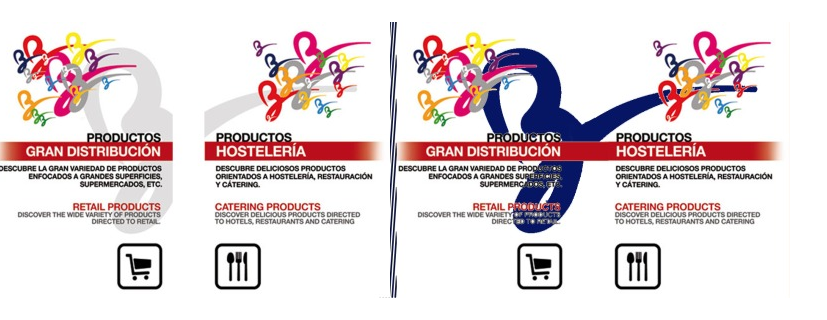
\includegraphics[scale=0.40]{principio-cont-2.png}
        \caption{Principio de continuidad en la página de Bornay Desserts}
    \end{figure}

    En esta figura se ha separado mediante una línea vertical de color azul la imagen central original con su hueco central, de la imagen de lo que el usuario percibe, destacando en color azul la B completa y con color granate el hueco de la línea central. El usuario percibe estos elementos unidos aunque están interrumpidos.
\end{itemize}

\subsubsection{Principio de Cierre y de Tamaño Relativo}
Estos principios establecen como nuestro cerebro ve figuras cerradas a partir de contornos y como se perciben dos objetos de distinto tamaño superpuestos.

\begin{itemize}
    \item \textbf{Principio de Cierre}

    Nuestra mente tienda a percibir figuras completas o cerradas a partir de contornos, incluso aunque éstos estén incompletos. En la siguiente imagen podemos ver un ejemplo.

    \begin{figure}[H]
        \centering
        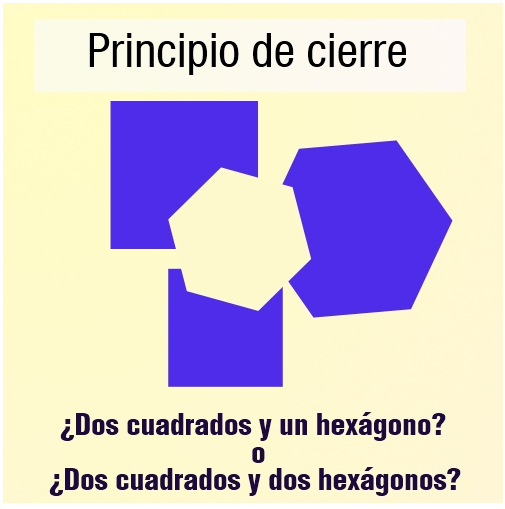
\includegraphics[scale=0.40]{principio-contor-1.png}
        \caption{Principio de cierre de Gestalt}
    \end{figure}

    Un ejemplo de la aplicación de este principio lo puede ver en las tres zonas enmarcadas con un rectángulo grisáceo en la parte derecha de la siguiente imagen. La parte izquierda se corresponde con el aspecto original de la página web de la empresa Endesa Logística S.L.

    \begin{figure}[H]
        \centering
        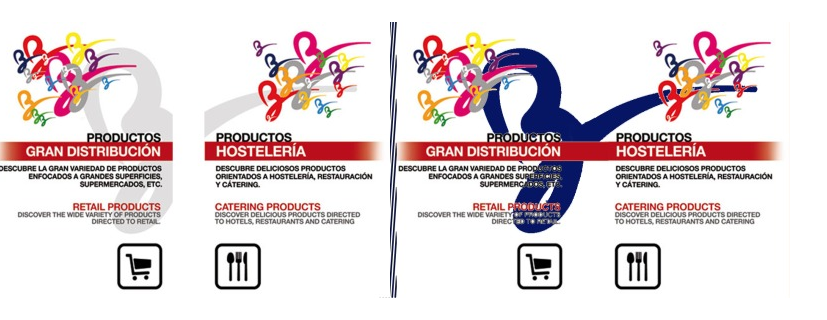
\includegraphics[scale=0.40]{principio-cont-2.png}
        \caption{Aplicación del principio de cierre en una web}
    \end{figure}

    \item \textbf{Principio de Área o Tamaño Relativo}

    Este principio estipula que nuestra mente tiende a percibir como objeto el más pequeño de dos objetos superpuestos, percibiendo el objeto de mayor tamaño como fondo. En la siguiente imagen vemos un ejemplo de este principio.

    \begin{figure}[H]
        \centering
        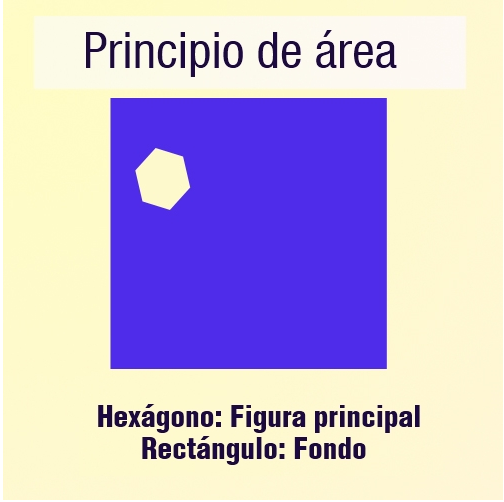
\includegraphics[scale=0.40]{principio-cierre-1.png}
        \caption{Principio de cierre de Gestalt}
    \end{figure}

    El hexágono se ve como la figura principal de la imagen y el cuadrado azul se percibe como el fondo sobre el cuál se encuentra el hexágono. En la siguiente imagen, podemos ver un ejemplo de aplicación de este principio.

    \begin{figure}[H]
        \centering
        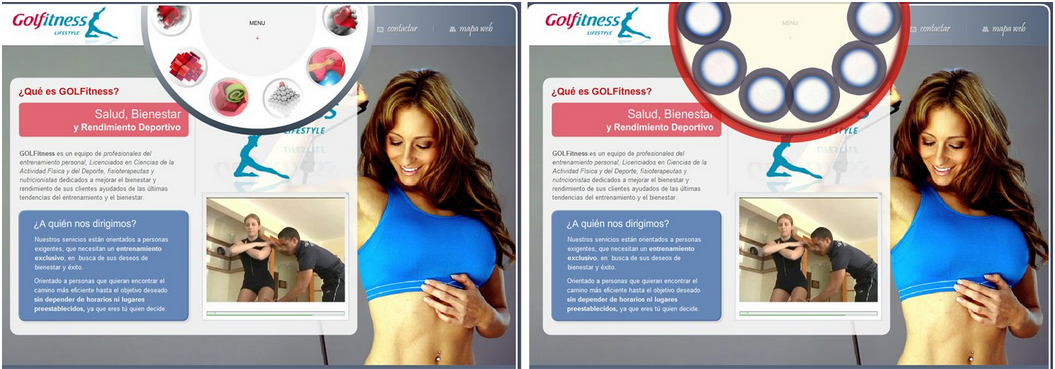
\includegraphics[scale=0.40]{principio-cierre-2.png}
        \caption{Aplicación del principio de cierre en una página web}
    \end{figure}

    Podemos ver el principio aplicado en las zonas enmarcadas mediante círculos en la parte derecha de la imagen. La circunferencia roja representa el fondo y los círculos pequeños son los elementos de interés. La parte izquierda de la imagen se corresponde con el aspecto original de la página web de la empresa Golfitness Style, donde se pueden ver las imágenes que están debajo de los círculos y que corresponden con la zona de navegación.
\end{itemize}

\subsubsection{Principio de Figura-Fondo}
Nuestra mente tiende a percibir ciertos elementos como figuras, con forma y borde, destacándolos del resto de los objetos que los envuelve. En la siguiente imagen puedes ver un ejemplo de este principio.

\begin{figure}[H]
    \centering
    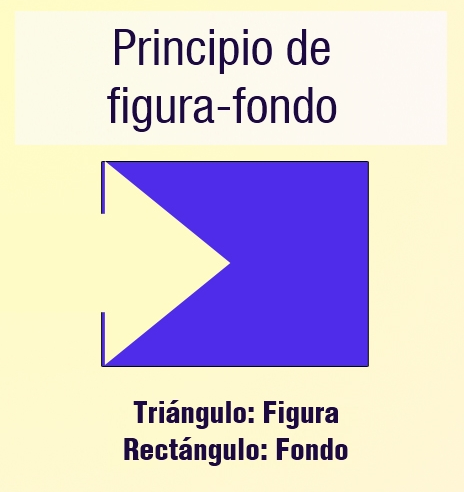
\includegraphics[scale=0.40]{principio-fig-1.png}
    \caption{Principio de figura-fondo de Gestalt}
\end{figure}

En la imagen distinguimos en triángulo de color claro como una imagen sobre el rectángulo de color azul que está de fondo, debido a que asimilamos mejor la forma triangulas que la poligonal. Si esto no fuera así, estaríamos viendo un triángulo a la izquierda y un polígono a la derecha.


\begin{figure}[H]
    \centering
    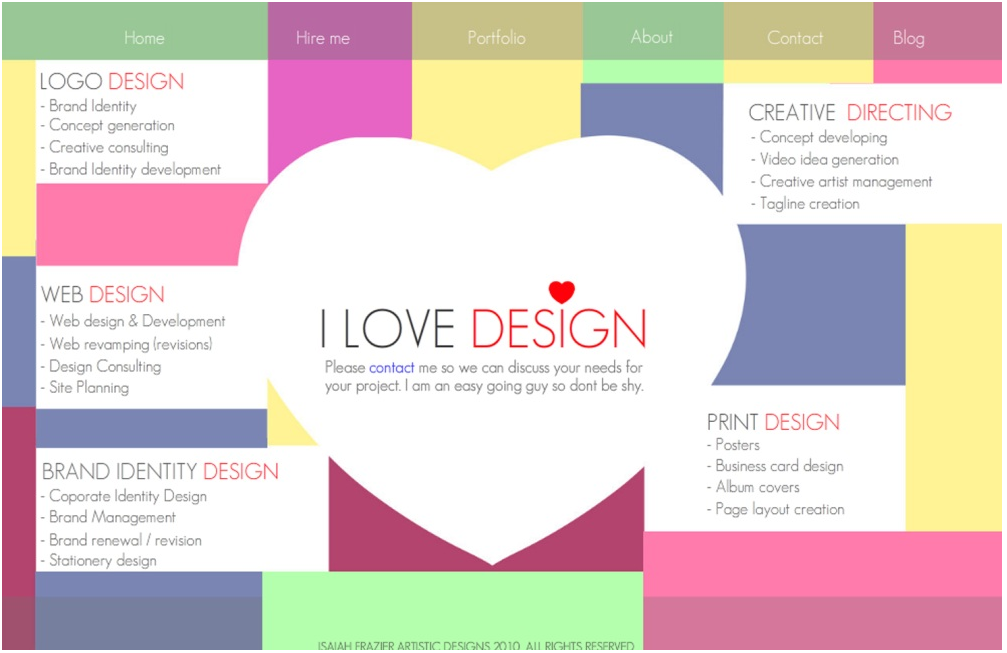
\includegraphics[scale=0.40]{principio-fig-2.png}
    \caption{Aplicación del principio figura-fondo en una web}
\end{figure}

Un ejemplo de aplicación de este principio es la imagen de la página de Isaiah Fraizer Artistic Designs. En ella podemos ver el corazón como un objeto principal situado sobre un fondo de rectángulos de colores.

\subsubsection{Ley de Simplicidad, Pregnancia o Buena Forma}
La \textbf{ley de simplicidad} establece que nuestra mente tiende a percibir las formas más simples, facilitando así su recuerdo. Es un principio de organización de los elementos que componente nuestra experiencia perceptiva, por el cual se reducen las ambigüedades o efectos distorsionadores, permitiéndonos centrarnos en un objeto separándolo del entorno con facilidad.


\begin{figure}[H]
    \centering
    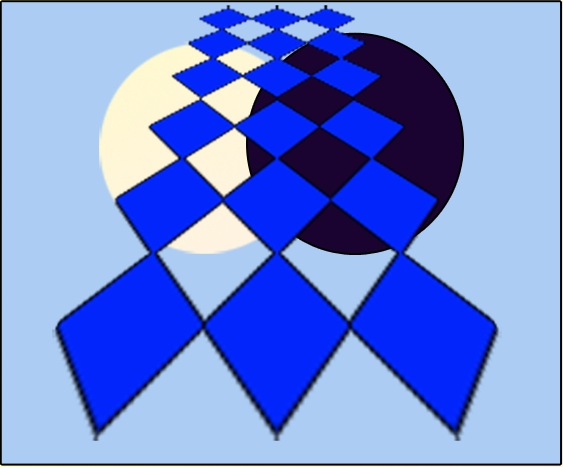
\includegraphics[scale=0.30]{principio-simp-1.png}
    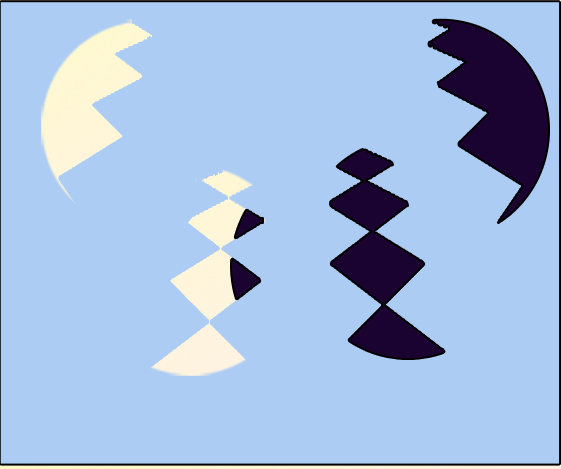
\includegraphics[scale=0.30]{principio-simp-2.png}
    \caption{Ley de simplicidad de Gestalt}
\end{figure}

En la figura de la izquierda nuestra mente percibe un circulo de color blanco y otro azul aunque estén colocados detrás de los rombos. No percibe las figuras que podemos observar en la imagen de la derecha, las cuales se han separado a propósito para evitar la percepción inevitable de la forma.

La misma imagen que poníamos como ejemplo del principio figura-fondo nos vale como aplicación práctica de otros principios. Distinguimos en la fila superior los elementos que forman parte del sistema de navegación por la tonalidad más oscura de los colores (\textbf{principio de semejanza}). También hay agrupación de elementos en distintos rectángulos con fondo blanco (\textbf{principio de proximidad}). Y vemos rectángulos completos incluso cuando están cortados por la silueta del corazón blanco (\textbf{principio de cierre}).

\begin{figure}[H]
    \centering
    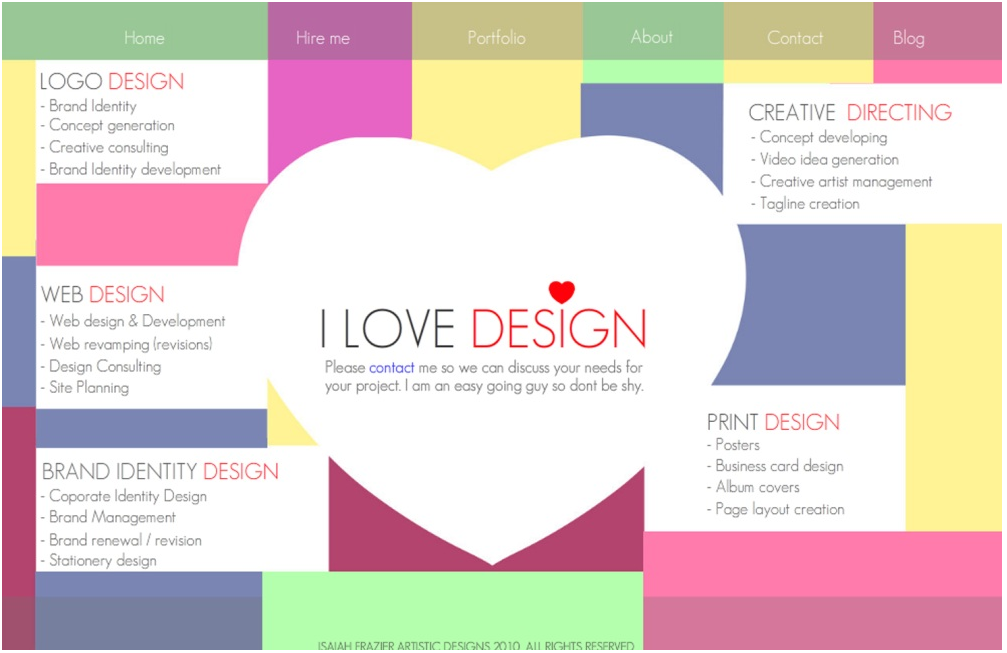
\includegraphics[scale=0.30]{principio-fig-2.png}
    \caption{Aplicación de varios principios de Gestalt}
\end{figure}

En los \textbf{sitios Web } es fundamental \textbf{conseguir un equilibrio} de los elementos que conforman la interfaz, hasta tal punto, de que esta logre pasar desapercibida por el usuario. Esta paradoja de buscar lo imperceptible usando principios fundados en la percepción, nos lleva a comprender la importancia de realizar un \textbf{diseño centrado en el usuario} y no en nuestros gustos personales. Es necesario que el usuario se familiarice lo más rápido posible que sea con nuestra interfaz. Nos apoyamos en los principios de Gestalt en un intento de lograr nuestros objetivos, \textbf{diseñar} una \textbf{interfaz usable} y además \textbf{visual}.

\subsection{El Color}
El color\textbf{} es un \textbf{aspecto esencial} en el diseño Web. Una elección inadecuada de los colores puede ser motivo para la pérdida de visitantes. En este punto, hablaremos de lo que deberíamos tener en cuenta a la hora de seleccionar los colores de nuestro sitio Web.

\begin{figure}[H]
    \centering
    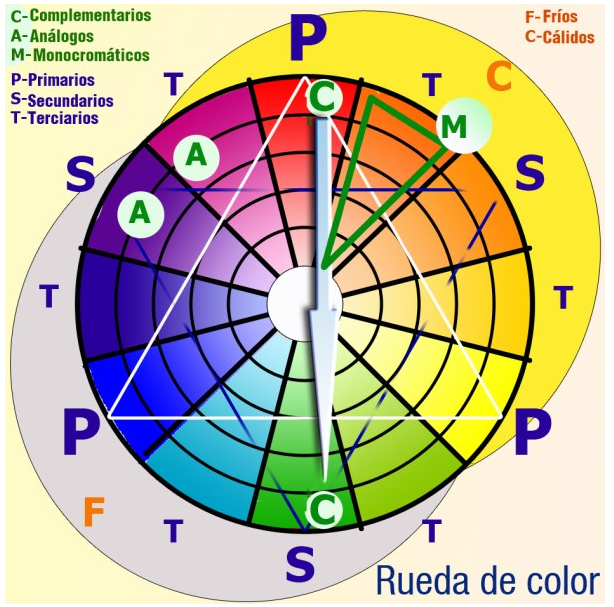
\includegraphics[scale=0.40]{rueda-color.png}
    \caption{Rueda de Color}
\end{figure}

Los colores están relacionados entre sí. La \textbf{rueda de color} formada por 12 colores es una herramienta gráfica importante para crear combinaciones cromáticas y que nos permite hacer distintas clasificaciones de los colores. Así, podemos clasificar los diferentes colores según las siguientes características:

\begin{itemize}
    \item \textbf{Colores Primarios}, \textbf{Secundarios} y \textbf{Terciarios}

    \begin{itemize}
        \item \textbf{Colores primarios}: hay tres colores primarios, estos son el \textbf{rojo}, \textbf{amarillo} y \textbf{azul}, y están dispuestos en la rueda formando un triángulo equilátero.

        \item \textbf{Colores secundario}: en la lado opuesto de la rueda a cada uno de los colores primarios se encuentran los colores secundarios, que son \textbf{verde}, \textbf{púrpura} y \textbf{naranja}. Cada uno de los colores secundarios se consigue con una mezcla de los dos sus dos colores primarios adyacentes. Así, el verde viene la mezcla del amarillo y el azul, el naranja, de la mezcla de rojo y amarillo, y el púrpura, de la mezcla de rojo y azul. Los tres colores secundarios forman también un triángulo equilátero.

        \item \textbf{Colores terciarios}: por último están los 6 colores terciarios, que son los que se consiguen al mezclar el color primario y el color secundario adyacentes al mismo. Así tenemos azul-verdoso, amarillo-anaranjado,  rojo-anaranjado, rojo-púrpura y azul-púrpura.
    \end{itemize}

    \item \textbf{Colores Fríos y Cálidos}
    \begin{itemize}
        \item \textbf{Colores fríos}: son colores fríos todos los situados, en la rueda de color, entre el amarillo-verdoso y el púrpura.

        \item \textbf{Colores cálidos}: son colores cálidos todos lo situados en la rueda de color entre el rojo-púrpura y el amarillo.
    \end{itemize}

    \item \textbf{Colores Complementario, Análogos y Monocromáticos}
    \begin{itemize}
        \item \textbf{Colores complementarios}: son aquellos colores que están en lados opuestos de la rueda cromática. Se utilizan para \textbf{crear contraste}.

        \item \textbf{Colores análogos}: son aquellos colores que se encuentran juntos en la rueda cromática. Se suelen usar para \textbf{crear armonía del color}.

        \item \textbf{Colores monocromáticos}: son todos los tonos y matices de un mismo color.
    \end{itemize}
\end{itemize}

En \href{https://paletton.com/#uid=1000u0kllllaFw0g0qFqFg0w0aF}{este enlace}, puedes encontrar una herramienta, \textbf{Paletton}, que nos va a ayudar a ir probando lo que vamos a estudiar en este punto sobre el color, además, de en un futuro, para que puedas elegir los colores para tu sitio web.

\subsubsection{El Sistema RGB}
El ojo humano percibe los colores rojo, verde y azul, y el resto de colores se realiza se consigue con la adición de estos tres colores en diferentes proporciones. El blanco se consigue con la mezcla de los tres colores puros y el negro se considera la ausencia total de color.

A estos colores se les conoce como \textbf{colores aditivos} y el ordenador se basa en este sistema para representar los colores, dando lugar a lo que conocemos como \textbf{Modo de color RGB}. RGB es el acrónimo de los colores rojo, verde y azul en inglés (Red Green Blue).

Los \textbf{ordenadores emplean estos tres colores} para representar cualquier colore de la escala cromática. Para ello, utilizan 8 bits de información para representar cada color. La escala monocromática de un color viene dada por todas las posibles combinaciones de estos 8 bits, es total\textbf{ 256 combinaciones}. Si tenemos en cuenta que tenemos una escala de 0 a 255 para representar cada color, es decir, 256 grados de color, y que el resto de los colores se consigue mezclando estos tres, ¿cuantos colores tenemos en total? Para saberlo, debemos de calcular todas las combinaciones posibles multiplicando 3 veces el número de grados que tenemos, es decir:

\begin{equation*}
    256\;x\;256\;x\;256 = 16.777.216
\end{equation*}


Es decir, con este sistema tenemos \textbf{16.777.216 de colores} usando 8 bits para representar cada uno de los colores aditivos. A la hora de representar cada color, usamos este modelo RGB y lo podemos expresar tanto en el sistema de numeración decimal como en hexadecimal.

\begin{figure}[H]
    \centering
    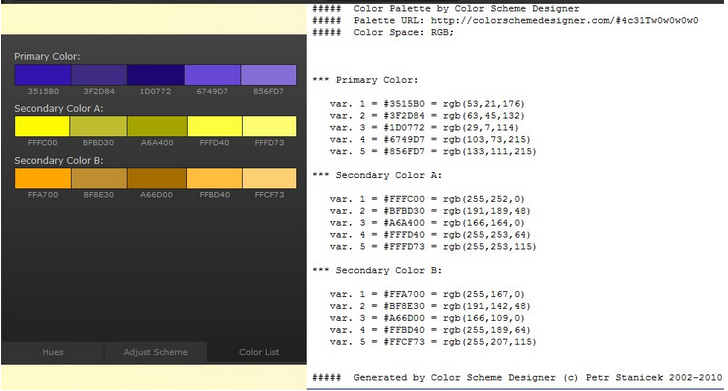
\includegraphics[scale=0.50]{esquema-rgb.png}
    \caption{Esquema RGB}
\end{figure}

En la imagen puedes ver las diferentes informaciones suministradas por la página web sobre esquemas de colores que compartimos como enlace en el punto anterior. Se ha elegido en el sistema RGB una tríada compuesta por un color primario, el azul, y los equidistantes a su color complementario. Se pueden ver los códigos hexadecimales correspondientes a cada combinación de color y en la parte derecha, sobre fondo blanco, la equivalencia en decimal de esos códigos hexadecimales.

\subsubsection{Colores Seguros}
El color rojo siempre será rojo, pero es posible que quede algún usuario con un monitor antiguo o con una versión del navegador muy anticuada, y debemos tenerlo en cuenta.

Hay monitores que solo permiten visualizar 256 colores, o navegadores que solo soportan 216, conocimos en el ámbito del diseño como c\textbf{olores seguros}. Emplear estos colores seguros es una forma de garantizar que nuestro sitio Web se verá igual en todos los navegadores.

Los \textbf{colores seguros} son los que se forman con las \textbf{combinaciones} de los tres colores \textbf{rojo}, \textbf{verde} y \textbf{azul}, pero solo con los valores hexadecimales \textbf{00}, \textbf{33}, \textbf{66}, \textbf{99}, \textbf{CC} y \textbf{FF}. Son 6 grados distintos de cada color y de ahí que sean \textbf{216 colores en total}.

\begin{figure}[H]
    \centering
    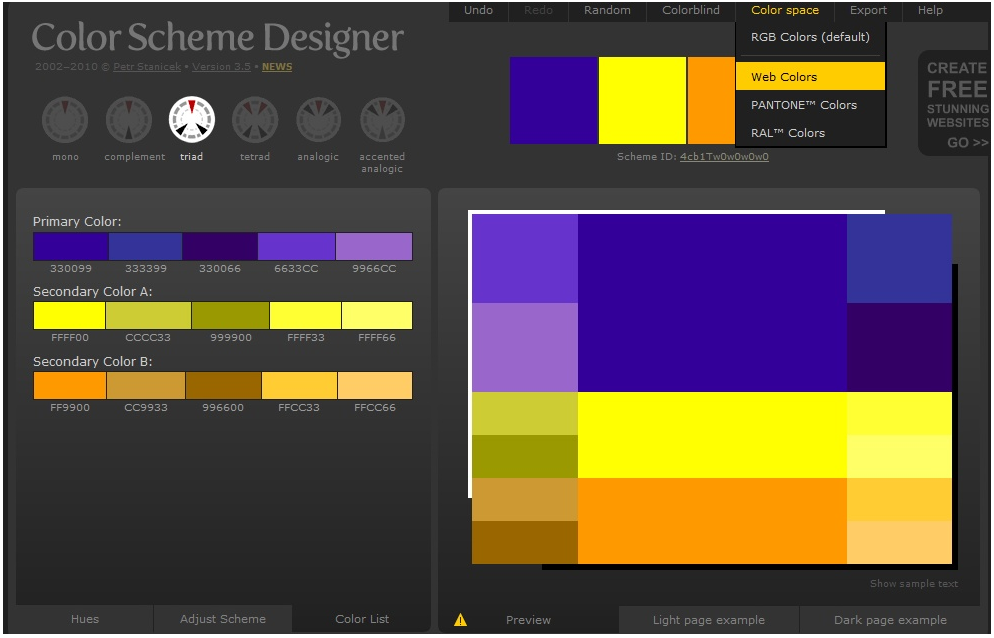
\includegraphics[scale=0.50]{secure-colors.png}
    \caption{Selección colores seguros}
\end{figure}

Como vemos en la imagen, hemos seleccionado los colores seguros de la Web, seleccionando la opción en el menú superior de la herramienta. Puedes comprobar que todos los códigos hexadecimales se corresponden con los mencionados en el párrafo anterior.

Para terminar esta sección, te recomendamos que consultes \href{https://www.testking.com/techking/wp-content/uploads/2011/01/IG-PoC-1000px.jpg}{este enlace} donde podrás ver un esquema con a modo de resumen explicando la \textbf{psicología del color}, que nos ayudará también a seleccionar los colores de nuestro sitio Web según la sensación que queramos transmitir.

\section{Generación de Documentos y Sitios Web}
Cuando diseñamos un sitio Web tenemos que tener claro que es tan importante el resultado final, el visual, lo que ve el usuario, como todo el trabajo previo de diseño y toda la documentación que habrá que realizar durante este proceso.

Como cualquier proyecto de software, el proceso de generación de un sitio Web para por \textbf{diferentes fases}, siendo estás más o menos complejas dependiendo del sitio que estemos desarrollando. Estas fases son:

\begin{itemize}
    \item \textbf{Análisis}: en esta fase, después de recabar la información necesaria, establecemos los \textbf{requisitos} que deberá cumplir la Web, su sistema de navegación y su funcionalidad, y se \textbf{eligen las herramientas} necesarias y los \textbf{lenguajes} con los que estará implementado el sitio Web. También se \textbf{establecen unas pautas} que todos los miembros del equipo de diseño deberán tener en cuenta durante la generación del sitio y durante su mantenimiento. Estas pautas incluyen: tipografía, colores, iconografía, distribución de los elementos, etc.

    \item \textbf{Desarrollo}: en esta fase se emplean las herramientas y lenguajes seleccionados en la fase anterior y se \textbf{implementa} el sitio Web, atendiendo a las pautas definidas en la fase de análisis.

    \item \textbf{Pruebas y Depuración}: en esta fase, que se debe ir realizando de forma \textbf{paralela al desarrollo}, se comprueba que todos los enlaces funcionan y que los usuarios pueden ir interactuando correctamente con todas las páginas del sitio. Es importante ir probando que el diseño ya realizado es operativo.

    \item \textbf{Documentación}: esta fase se realiza de \textbf{forma paralela a las demás}. Hay que documentar los requisitos establecidos en la fase de análisis. También hay que documentar el código durante la fase de implementación para facilitar su posterior mantenimiento. Pero lo más importante en el diseño Web es, quizás, la documentación de las pautas a seguir durante la generación del sitio. Estas pautas, recogidas en una \textbf{guía de estilo}, servirán al equipo de diseño durante la generación y mantenimiento del sitio.
\end{itemize}

\subsection{Guías de Estilo y sus Elementos}
Un \textbf{manual de estilo} es un conjunto de normas para el diseño y redacción de documentos, ya sea para el uso general, o para una publicación u organización específica. Los manuales de estilo son frecuentes en el uso general y en el especializado, en medios escritos, orales o gráficos. El manual de estilo se compone tanto de normas lingüísticas, como de estilo, para que el mensaje sea más coherente, eficaz y correcto.

Algunos manuales se centran en el diseño gráfico y abarcan temas como la tipografía, los colores y espacios en blanco. Los \textbf{manuales de estilo de sitios Web} se centran en los aspectos técnicos y visuales de la publicación, la prosa, uso correcto del lenguaje, la gramática, puntuación, la ortografía, pero sobre todo, la estética. La estricta aplicación de los manuales de estilo proporciona uniformidad al aspecto visual de un documento.

La \textbf{guía de estilo} esta dirigidas a personas que se encargan del diseño y programación de la interfaz Web. Esta guía debe recoger todos los aspectos relacionados con el diseño de la interfaz y servir de ayuda eficaz en la toma de decisiones, tanto en el proceso de diseño como posteriormente en el proceso de mantenimiento.

Una guía de estilo incluye aspectos relacionados con la inclusión en la interfaz de fotografías, logos, imágenes, iconos, los colores, los tipos de letra y, aquellos relacionados con la maquetación Web. Cuando una web esta desarrollada por un grupo de personas, la guía de estilo se hace \textbf{imprescindible}.

Es recomendable que visites los siguientes enlaces donde podemos ver diferentes guías de estilo de varias instituciones y sitios web.

\begin{itemize}
    \item \href{https://si.ua.es/es/web-institucional-ua/guia-de-estilo.html}{Guía de estilo de la Universidad de Alicante}
    \item \href{http://www.upv.es/entidades/ASIC/manuales/guia_estilos_upv.pdf}{Guía de estilo de la Universidad de Valencia}
\end{itemize}

\subsubsection{Fotos y Logos}
Los recursos gráficos son muy empleados en la Web. Si se usan correctamente, pueden añadir valor a esta y facilitar el aprendizaje del usuario. Pero si se usan incorrectamente, pueden tener el efecto contrario.

A la hora de emplear imágenes hay que tener en cuenta que estas son archivos que \textbf{tienen un tamaño}, y por tanto, \textbf{deberán descargarse} antes de su visualización. Por ello, solo \textbf{usaremos imágenes} que \textbf{complementen} nuestros sitio Web y trataremos de evitar aquellas cuya única finalidad sea adornas el sitio. Sobre las imágenes hablaremos en la unidad 5 en más profundidad.

A continuación vemos una imagen ilustrativa de diferentes elementos que se han usado en otros apartados y que entran dentro de la categoría de fotos y logos.

\begin{figure}[H]
    \centering
    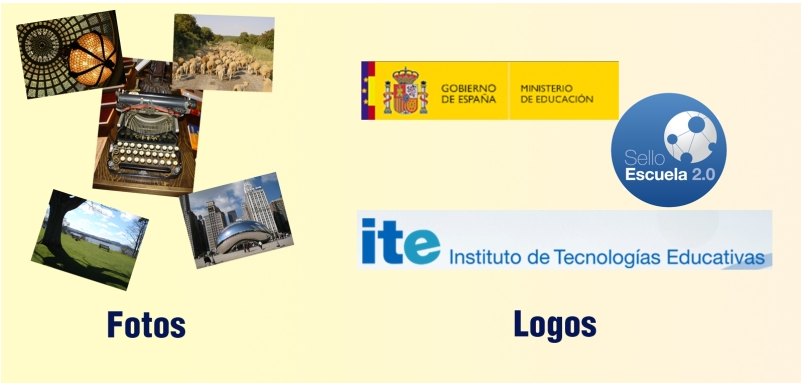
\includegraphics[scale=0.50]{fotos-logos.png}
    \caption{Fotos y logos}
\end{figure}

Ahora lo que nos importa es la información que se debe reflejar en una guía de estilo referente a estos elementos, en los que deben figurar los siguientes puntos:

\begin{itemize}
    \item \textbf{Formato}: el tipo de formato en el que deberán estar almacenadas las imágenes o logotipos empleados.
    \item \textbf{Tamaño}: el tamaño de logotipo o imagen que se establece dando las medias de ancho y alto en píxeles.
\end{itemize}

Hay que tener en cuenta demás que se \textbf{deben incluir} todos los \textbf{tamaños posibles} que puedan tener la imágenes o logotipos según su funcionalidad o en lugar de la página donde deberán ir situados, ya que no es lo mismo una imagen que vaya en la zona de contenidos que una imagen que se use en la cabecera de una página como distintivo de la organización.

\textbf{Todos los tamaños y formatos} a emplear por el equipo deben quedar \textbf{perfectamente descritos} en el documento de la guía de estilo.

\subsubsection{Tipografías}
La \textbf{elección de la tipografía} es otro elemento muy importante en el diseño de una Web. La elección de una fuente familiar para el usuario puede facilitar la lectura y añadir valor al sitio Web.  A la hora de elegir la tipografía más adecuada tenemos que tener en cuenta lo siguiente:

\begin{itemize}
    \item \textbf{La fuente}: no todas las fuentes se leen con la misma facilidad y no todas las fuentes se ven igual en todas las plataformas. La fuente \textbf{Arial} es una fuente muy extendida que asegura la correcta visibilidad en todos los tamaños y en todas las plataformas y navegadores.

    \item \textbf{El estilo de la fuente}: en la guía de estilo hay que especificar en que casos usar negrita, cursiva, subrayado o alguna de las posibles combinaciones. Hay que tener en cuenta que:

    \begin{itemize}
        \item El \textbf{subrayado} se suele emplear normalmente en los \textbf{enlaces}, pudiendo dar una falsa impresión al usuario si se emplea con otra finalidad.
        \item Se debe usar \textbf{negrita} solo para conseguir fijar la atención del usuario sobre un elemento, destacándolo del resto.
        \item No se deben utilizar diferentes características de la fuente para mostrar el énfasis de mas de una o dos palabras o una frase corta.
    \end{itemize}

    \item \textbf{Tamaño de la fuente}: la guía de estilo debe reflejar los tamaños de la fuente en función de la ubicación del texto y su finalidad. No se emplea el mismo tamaño del texto para un titular que para su contenido. Así mismo, se pueden establecer diferentes tamaños según la importancia del titular.

    \item \textbf{Color de la fuente}: la guía de estilo debe especificar el color de la fuente en función de la ubicación del texto y su finalidad. A la hora de elegir el color debemos tener en cuenta lo siguiente:

    \begin{itemize}
        \item Se lee mejor el texto en color oscuro sobre un fondo blanco que al revés.
        \item Se lee mejor un texto sobre un fondo liso que sobre un fondo con alguna textura o con una imagen.
    \end{itemize}

    Conocer lo \textbf{distintos tipos de fuentes} y \textbf{su comportamiento} en diferentes navegadores y sistemas operativos es de gran importancia para garantizar una visualización consistente de nuestro sitio Web.

    Por último, dejamos un enlace con los \href{https://mejoratucopy.com/tipografias-para-web/}{tres mandamientos} que debe cumplir la tipografía de nuestra web.
\end{itemize}

\subsubsection{Colores}
En una guía de estilo deben figurar todos los colores que se van a usar en todos los textos, fondos e imágenes según sea su ubicación y finalidad. La información debe suministrarse aportando los valores RGB tanto en decimal como en hexadecimal.

\begin{figure}[H]
    \centering
    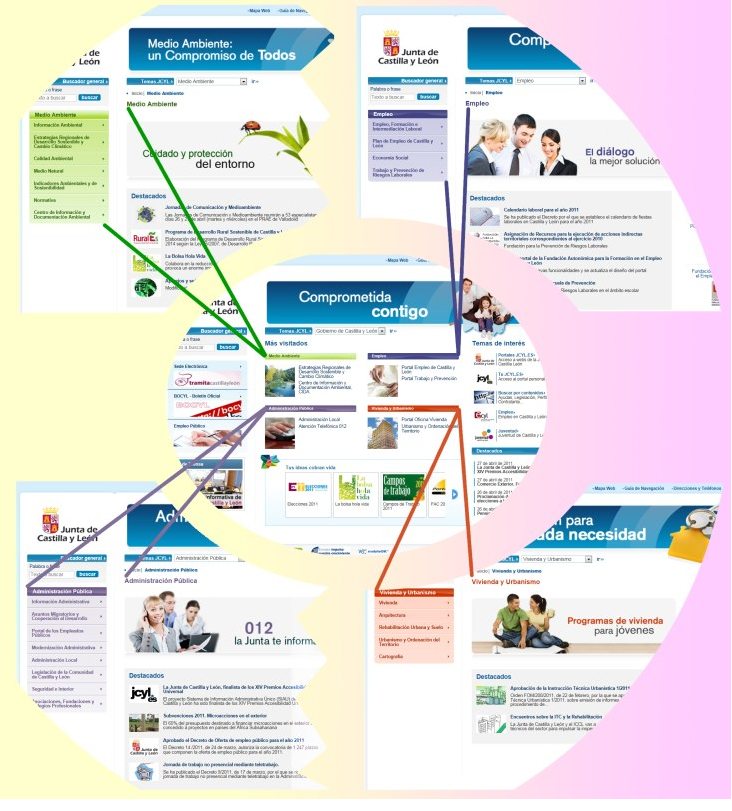
\includegraphics[scale=0.33]{guia-colores.png}
\end{figure}

En muchos sitios se usan colores distintos en los distintos enlaces del sistema de navegación de su página principal. Estos mismo colores se emplean después para representar otras secciones del sitio. Por ejemplo, en el sitio de la Junta de Castilla  y León tiene en su parte centra una zona de navegación enlazada con las secciones más visitadas:

\begin{itemize}
    \item Medio ambiente: tiene una fuente de color verde oscuro sobre un fondo de color verde claro.
    \item Empleo: tiene la fuente de color blanco sobre un fondo de color oscuro.
    \item Administración pública: tiene una fuente de color blanco sobre un fondo de color púrpura.
    \item Vivienda y Urbanismo: tiene la fuente de color blanco sobre un fondo de color rojo.
\end{itemize}

Cada una de las secciones utiliza los mismos colores o algunos de su misma escala en su zona de navegación y en el título del contenido propio de sección. En este caso, la guía de estilo debe reflejar, entre otras, las combinaciones hexadecimales para el color de:

\begin{itemize}
    \item Las fuentes en el bloque central de la página.
    \item Los fondos de los títulos de las secciones de la página principal.
    \item Las fuentes del menú de navegación y el título del contenido en cada una de las páginas de las secciones.
    \item Los fondos de las opciones del menú de navegación y de su título en cada una de las páginas de las secciones.
\end{itemize}

Por último, aquí te dejamos \textbf{unos consejos} que te pueden ser útiles a la hora de seleccionar los colores de tu sitio Web:

\begin{itemize}
    \item Si vas a emplear colores como \textbf{sistema de codificación}, es decir, para que el usuario haga una distinción de finalidad de los elementos según su color, asegúrate de que sea \textbf{fácil de comprender}.
    \item \textbf{Ser consistente }en el uso de colores, usando por ejemplo un color siempre para lo mismo.
    \item \textbf{No excederse} en el uso de colores distintos.
    \item Utilizar combinaciones de colores que \textbf{trasmitan armonía}.
    \item Utilizar correctamente el \textbf{contraste de colores} para destacar las partes relevantes del sitio.
    \item Ten en cuenta la \textbf{psicología del color}.
\end{itemize}

\subsubsection{Iconografía}
La \textbf{iconografía} es la aplicación práctica de los elementos prácticos del diseño (Representación, Significado y Función). Según la Real Academia Española, un icono es un signo que mantiene una relación de semejanza con el objeto representado.

La Wikipedia dice que, desde el punto de vista informático, \textbf{un icono} es un pequeño elemento gráfico en pantalla que identifica y representa algún objeto, usualmente con algún simbolismo gráfico, para establecer una asociación.

Un icono es una aplicación del elemento \textbf{Representación} porque es una forma representativa de algo en el mundo real; es una aplicación del elemento \textbf{Significado} porque el mensaje transmitido por el icono genera en nuestra mente una imagen conceptual, y es una aplicación del elemento \textbf{Función} porque logra atraer la atención del usuario que percibe de una forma más rápida el mensaje que se intenta transmitir y de esta forma no tiene necesidad de leer el texto al que acompaña.

Los iconos suelen emplease para completar los textos de los enlaces en la página de portada. Un icono debe contener la \textbf{menor cantidad de detalle} posible sin perder significado.

La elección de los iconos es muy importante, puesto que si un usuario no es capaz de determinar su significado a simple vista, entonces no habremos conseguido nuestro propósito de ahorrarle tiempo en la visualización de la página.ç

\begin{figure}[H]
    \centering
    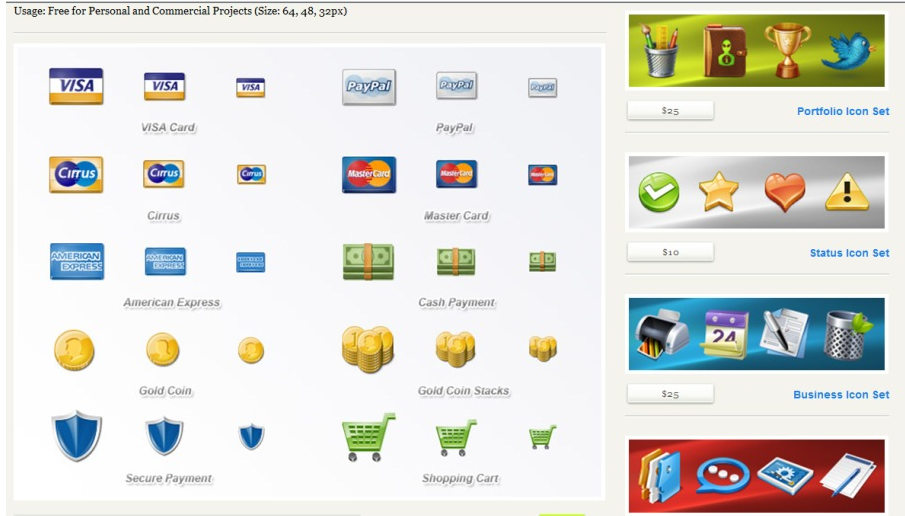
\includegraphics[scale=0.40]{iconos.png}
    \caption{Ejemplos de iconos}
\end{figure}

En la imagen podemos ver iconos agrupados según su ámbito de aplicación. En el grupo más grande los iconos están relacionados con el comercio: tarjetas de crédito, monedas, billetes, etc. Estos icono y otros con un diseño parecido son de uso común en todos los sitios web on-line.

En la guía de estilos se deben especificar los iconos a emplear en el sitio Web, donde se van emplear y con que finalidad. Usar iconos por el mero hecho de adornar nuestra Web pero que no importe su significado es algo arriesgado.

\subsubsection{Estructura}
En el apartado de \textbf{Maquetación Web} hablábamos de la disposición de los bloques de elementos dentro del espacio de la ventana del navegador y veíamos un ejemplo de distribución de dichos elementos muy empleada en los diseños de interfaces Web.

En el apartado de \textbf{Mapas de Navegación} hablábamos también de la relación existente entre las páginas a través de sus enlaces.

En la \textbf{guía de estilos} debe quedar reflejada no solo la disposición de estos bloques en cada una de las páginas Web de nuestro sitio, sino también la relación de navegación entre las diferentes páginas.

Es muy común en los sitios Web de gran tamaño que la \textbf{página principal} tenga una \textbf{diseño diferente} al resto de páginas, pero tanto si todas las páginas son iguales como si tenemos tanto si tenemos grupos de páginas iguales entre sí, la guía debe reflejar todos los diseños posibles indicando en todos los casos:

\begin{itemize}
    \item El tamaño en píxeles o porcentaje que debe ocupar \textbf{el encabezado} y dentro de él lo que ocupara y donde se ubicará cada uno de sus elementos.
    \item El tamaño en píxeles o porcentaje de la \textbf{zona de navegación} y su ubicación, así como si estará dispuesta de forma horizontal u vertical.
    \item Como se \textbf{dispondrán los enlaces} dentro de cada zona de navegación y su tamaño.
    \item El tamaño, lugar y formato de la \textbf{zona de posicionamiento} dentro de la página.
    \item El tamaño de la \textbf{zona de contenido} y su ubicación. Donde se colocará el título y lo que ocupará dentro de la zona de contenido.
    \item Si hay \textbf{cuadros de contenido secundario}, cuál va a ser su tamaño y posición, y cual será su funcionamiento. Si estarán visibles o se mostrarán al pasar el ratón por alguna zona concreta.
    \item El tamaño y la distribución de los \textbf{elementos de pie}.
    \item También se deberán reflejar los \textbf{huecos} que se dejaran a propósito.
    \item Como se van a mostrar los \textbf{submenús} de navegación.
\end{itemize}

\subsection{Aplicaciones Para El Desarrollo Web}
En este punto, vamos a conocer algunas de las herramientas que podemos emplear para desarrollar nuestro sitio Web, en especial, las que nos van a permitir crear los elementos gráficos, los contenidos y la maquetación de los mismos.

En \href{https://www.lawebera.es/}{este artículo de La Webera} puedes empezar consultando todas las herramientas que vas a necesitar para crear un sitio web. Aunque aquí vamos a ver algunas de estas.

Dada la infinidad de herramientas que disponibles, haremos una agrupación de las mismas y daremos el nombre de algunas que no figuran en el artículo de el enlace y que pueden ser interesantes. Si te vas a dedicar profesionalmente al diseño de aplicaciones Web y dentro de esta profesión de especializas en el diseño de interfaces, necesitaras conocer, al menos, algunas de las herramientas que vemos en la siguiente tabla.

\begin{figure}[H]
    \centering
    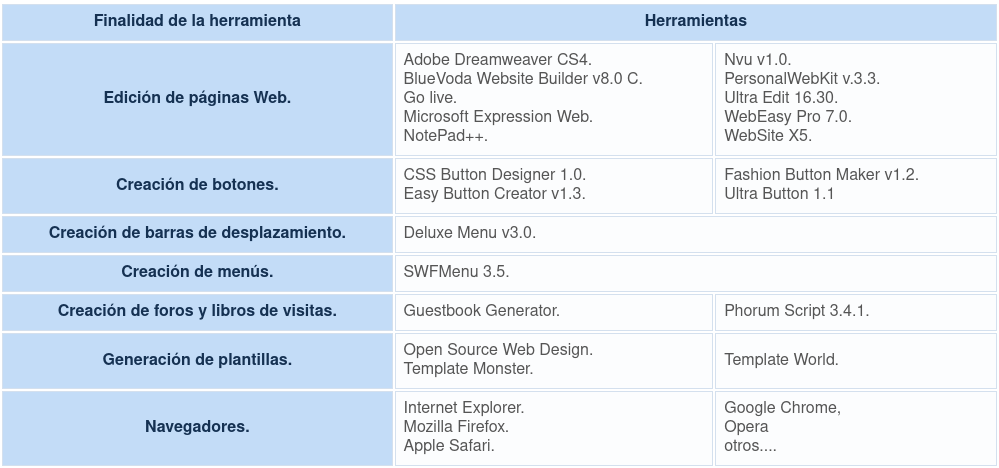
\includegraphics[scale=0.60]{tabla-herramientas.png}
\end{figure}

Las herramientas a emplear para la edición de imágenes, sonido, vídeo, animaciones y contenido se verán en sus correspondientes unidades de trabajo.

\subsection{Lenguajes de Marcar}
Los sitios web están compuestos de páginas que están escritas en algún lenguaje. Aunque algunas de las herramientas vistas en el punto anterior te permite comenzar a hacer una web sin conocimientos de estos lenguajes, solo conociendo la propia herramienta, si tu intención es dedicarte profesionalmente, deberás conocer, comprender y utilizar los \textbf{lenguajes de marcar}. Los principales que podemos encontrarnos son:

\begin{itemize}
    \item \textbf{HTML}: acrónimo del inglés HyperText Markup Language,  es el lenguaje de marcado predominante para la elaboración de páginas web. Los documentos escritos en este lenguaje sirven tanto para definir la estructura como el contenido de la página web.

    HTML emplea marcas o etiquetas dentro del documento para informar al navegador de que se va a representar en el documento y lo hace, normalmente, delimitando el texto entre dos etiquetas, una de apertura y otra de cierre, aunque también hay etiquetas no tienen una de cierre. Las etiquetas van encerradas entre corchetes angulares y tiene unas normas sintácticas que se deben respetar si queremos que el resultado mostrado en el navegador sea el deseado.

    Si no tienes conocimientos de HTML o quieres ponerlos al día, puedes visitar este \href{https://es.wikibooks.org/wiki/Lenguaje_HTML}{Curso de Introducción a HTMl}.

    \item \textbf{HTML5}: es la nueva versión de HTML, que ha evolucionado de la versión HTML 4.0.1. Esta nueva versión incorpora muchas etiquetas nuevas, pero nosotros nos centraremos en las denominadas como \textbf{etiquetas semánticas}, algunas de las cuales son: \textbf{header}, \textbf{nav}, \textbf{main}, \textbf{section}, \textbf{article}, \textbf{aside} y \textbf{footer}. Esta etiquetas nos permitirán organizar nuestra web dándole un significado por el simple hecho de utilizarlas. Así, por ejemplo, al utilizar la etiqueta \textbf{nav} estamos indicando que lo que se encuentra dentro es un bloque de navegación.

    A continuación, se muestra un ejemplo de código en HTML5:

    \begin{figure}[H]
        \begin{tcolorbox}[sharp corners, colback=yellow!30, colframe=white!20]
            \scriptsize
\begin{verbatim}
<!DOCTYPE html>
<html lang="en">
  <head>
    <meta charset="UTF-8">
    <title>Document</title>
  </head>

  <body>
    <!-- Comentarios del código -->
    <h1> ¡Hola mundo! </h1>
  </body>
</html>
\end{verbatim}
        \end{tcolorbox}
    \end{figure}

    \item \textbf{XML}: acrónimo del ingles eXtensible Markup Language, se propone como estándar para el intercambio de información estructurada entre diferentes plataformas. XML no es realmente un lenguaje en particular, sino que es un \textbf{metalenguaje }extensible desarrollado por el World Wide Web Consortium (W3C).

    A diferencia de HTML, donde los errores sintácticos no provocan errores en el navegador, XML es muy estricto en cuanto a sus normas sintácticas.

    \item \textbf{XHTML}: acrónimo del ingles eXtensible Hypertext Markup Language, es un lenguaje que utiliza las mismas etiquetas y atributos que HTML pero aplicando las reglas sintácticas de XML. En este \href{https://es.wikipedia.org/wiki/XHTML}{artículo de Wikipedia} puedes ver con más detalle las características de XHTML y sus diferencias con HTML.
\end{itemize}

\subsection{Tablas, Capas y Marcos}
En los comienzos de HTML, la única forma de estructura una página era mediante el uso de \textbf{tablas}. Para poder agrupar los contenidos en los diferentes bloques de encabezado, navegación, contenido y pie, había que anidar tablas dentro de otras y definir los tamaños de cada bloque dándoles valores absolutos o relativos a la altura o anchura de cada celda. Era fácil, aunque laborioso, pero se conseguía situar cada elemento en su sitio. Había que tener el código HTML bien indentado para no perderse en un maremágnum de \textbf{tr} y \textbf{td}.

Las nuevas versiones de los navegadores incorporan los \textbf{frames} o \textbf{marcos} que permiten estructurar la ventana del navegador en partes independientes entre sí, mostrando en cada una de estas partes una página HTML distinta. La ventaja del uso de marcos respecto a las tablas es que se pueden dejar zonas de la ventana visibles permanentemente, además, al estar separadas unas de otras según su funcionalidad resulta más fácil realizar el mantenimiento.

Actualmente, \textbf{no deben utilizarse} ni tablas ni marcos para realizar la maquetación de nuestra página web, ya que hay herramientas más nuevas y eficientes que estás dos.

Con la aparición de las \textbf{hojas de estilo}, las cuales no hay que confundir con las guías de estilo, se dejan de emplear tanto marcos como tablas, sustituyendo ambos por el uso de etiquetas \textbf{div} para definir bloques y las hojas de estilo para configurar la visualización de dichos bloques. Pero este tema tiene la suficiente entidad como para dedicarle más adelante un tema entero.

Como hemos visto en el punto anterior, con la aparición de HTML5, han surgido un nuevo conjunto de etiquetas y complementan y en algunos casos sustituyen a la etiqueta \textbf{div} y que además añaden significado semántico al contenido que hay en su interior.

\subsection{Plantilla de Diseño}
En el apartado de \textbf{Maquetación Web} vimos un ejemplo de distribución de los bloques en los que se estructura una página web. Nos solemos encontrar esta distribución en sitios Web que no son excesivamente complejos, donde solo hay una zona de navegación que esta siempre visible y una zona de contenidos donde se representa cada uno de los contenidos enlazados desde la zona de navegación.

Hay muchas distribuciones de los elementos de una página web, pero después de navegar horas y horas nos damos cuenta que muchos sitios distintos tiene una distribución similar. Esto es debido a que la \textbf{reutilización de código} es una técnica común que intenta ahorrar tiempo y energía, reduciendo el trabajo redundante.

Las \textbf{plantillas de diseño Web} son sitios web prediseñados que se pueden usar como base en un diseño Web y que permiten adaptarlo a las necesidades del diseñador de forma rápida y sencilla, ahorrando una gran cantidad de tiempo y dinero.

\begin{figure}[H]
    \centering
    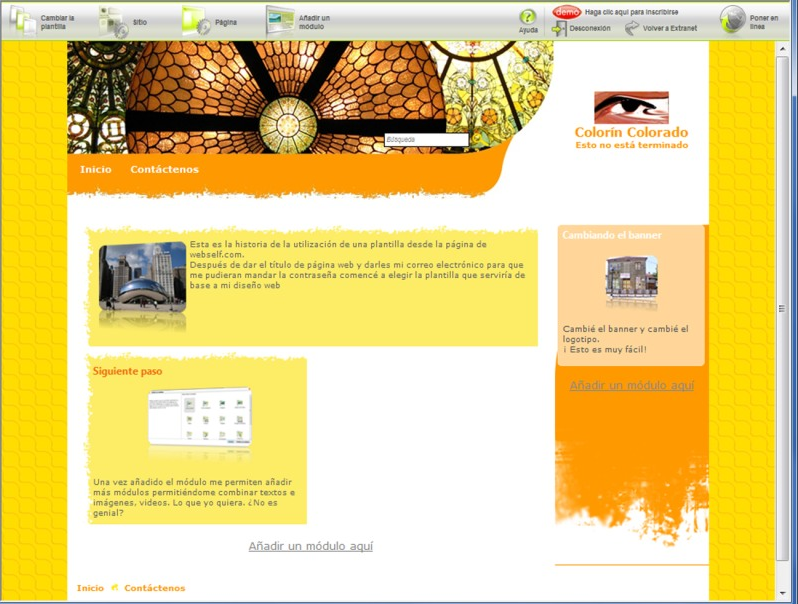
\includegraphics[scale=0.31]{diseno-plantilla.png}
\end{figure}

En la imagen anterior podéis ver un ejemplo de un diseño realizado en 20 minutos a partir de una plantilla suministrada por \href{https://www.webself.net/}{Webself}.

Hoy en día hay una gran cantidad de sitios comerciales que suministran plantillas de diseño Web por muy poco dinero si consideramos el tiempo ahorrado en el diseño. Además, la mayoría te dan alojamiento gratuito de tu sitio Web durante el primer año.

% Bibliography

\addcontentsline{toc}{chapter}{Bibliografía}
\bibliography{citas}
\bibliographystyle{unsrt}

\end{document}